\lstinputlisting[language=bash,basicstyle=\small]{python_codes/fieldstone_87/keywords}

\begin{center}
Code at \url{https://github.com/cedrict/fieldstone/tree/master/python_codes/fieldstone_87}
\end{center}

\par\noindent\rule{\textwidth}{0.4pt}

{\sl This stone was developed in collaboration with Riad Hassani}. \index{contributors}{R. Hassani}

\par\noindent\rule{\textwidth}{0.4pt}

%--------------------------------------------------------
\subsubsection*{The power law rheology}
\index{general}{Power Law Rheology}
\index{general}{Generalised Power Law Rheology}

In what follows the viscosity 
is assumed to be of the power law type, i.e.
\[
\eta(\dot{\bm \varepsilon}) = \beta  \dot{\varepsilon}_e^{\frac1n-1}
\]
where $\beta$ is a scalar, $n$ is a small number (but not 
necessarily an integer) and
$\dot{\varepsilon}_e$ is the effective strain rate defined in Eq.~\eqref{eq:tauepse},
i.e.
\[
\dot\varepsilon_e = \sqrt{ \frac{1}{2}(\dot\varepsilon_{xx}^2 + \dot\varepsilon_{yy}^2 ) 
+ \dot\varepsilon_{xy}^2}
\]
We will also consider the generalised power-law rheology:
\[
\eta_{\dot\gamma}(\dot{\bm \varepsilon})  = \beta  ( \dot{\varepsilon}_e^2 + \dot\gamma^2)^{\frac{1-n}{2n}}
\]
This formulation has the advantage that viscosity does not become infinite 
when the strain rate becomes zero.
Finally, to simplify notations we define $\alpha=\frac1n-1$ so that 
\[
\boxed{
\eta_{\dot\gamma}(\dot{\bm \varepsilon})  = \beta  ( \dot{\varepsilon}_e^2 + \dot\gamma^2)^{\alpha/2}
}
\qquad
\text{or simply}
\qquad
\boxed{
\eta(\dot{\bm \varepsilon})  = \beta  \dot{\varepsilon}_e^\alpha
}
\]


\Literature: Dynamics of strongly time-dependent convection
with non-Newtonian temperature-dependent viscosity, Larsen et al \cite{laym96}

 

%--------------------------------------------------------------------
\subsubsection*{Newton-Raphson method for single-valued functions}

Newton gave a version of the method in 1669. Raphson generalized and presented
the method in 1690. Both mathematicians used the same concept, and both algorithms gave the
same numerical results, which is why the method is often referred to as the Newton-Raphson method.


In numerical analysis, the Newton's method (also Newton-Raphson method) 
is an iterative root-finding algorithm.
The most basic version for a function $f(x)$ is as follows\footnote{\url{https://en.wikipedia.org/wiki/Newtons_method}}:
\[
x^{k+1} = x^k - \frac{f(x^k)}{f'(x^k)}
\]
where we assume that the derivative $f'$ exists and we start the iterations 
with a guess $x_0$.
If the function satisfies sufficient assumptions and the initial guess is close
to the real solution then the method converges to the root. 
Note that if a stationary point of the function is encountered, i.e. 
the derivative is zero, then the method will terminate due to division by zero. 

%--------------------------------------------------------------------
\subsubsection*{Newton-Raphson method for systems of equations}
Let us consider the following system of $N$ equations. 
\[
{\bm A} \cdot \vec{X} = \vec{b}
\]
Solving this system is equivalent to finding the root of 
\[
\vec{R}(\vec{X}) =  {\bm A} \cdot \vec{X} - \vec{b}
\]
i.e. finding the zeroes of the continuously differentiable function $\vec{R}: \R^N \rightarrow \R^N$. 
In this case, the Newton algorithm is written as a function of the $N\times N$ Jacobian 
matrix ${\bm J}_R$:
\begin{equation}
\vec{X}^{k+1} = \vec{X}^k - {\bm J}_R^{-1}(\vec{X}^k) \cdot {\vec R}(\vec{X}^k)
\end{equation}
or,
\begin{equation}
{\bm J}_R (\vec{X}^k) \cdot( \vec{X}^{k+1} - \vec{X}^k  )   = - \vec{R}(\vec{X}^k)
\label{eq:f87newt}
\end{equation}
where the Jacobian matrix is defined as follows\footnote{\url{https://en.wikipedia.org/wiki/Jacobian_matrix_and_determinant}}:
\[
{\bm J}_R = 
\left(
\begin{array}{ccc}
\frac{\partial R_1}{\partial X_1} & \dots & \frac{\partial R_1}{\partial X_N} \\
\vdots & \ddots & \vdots \\ 
\frac{\partial R_N}{\partial X_1} & \dots & \frac{\partial R_N}{\partial X_N} 
\end{array}
\right)
\]



%----------------------------------------------------------------
\subsubsection*{The super simple / no questions asked approach}


We have to solve 
\[
{\bm A}(\vec{X}) \cdot \vec{\cal X} = \vec{b}
\]
where the matrix ${\bm A}(\vec{\cal X})$ comes from the discretization of the incompressible
Stokes equations and the vector $\vec{b}$ corresponds to body forces, surface forces and 
boundary conditions. We assume here for simplicity that $\vec{b}$
is independent of the vector of unknowns $\vec{X}$, which is made of
$\vec{\cal V}$ and $\vec{\cal P}$. The dependence of ${\bm A}$ on $\vec{\cal X}$ 
comes from the dependence of the viscosity on strain rate (and therefore velocity)
and pressure (although in this particular case of the power law rheology pressure does 
not enter the equations). 

The matrix ${\bm A}(\vec{\cal X})$ has the following structure:
\begin{equation}
{\bm A}(\vec{\cal X}) = 
\left(
\begin{array}{cc}
\K(\vec{\cal X}) & \G  \\
\G^T & 0 
\end{array}
\right)
\end{equation} 
and the discretised Stokes system is then
\begin{equation}
\left(
\begin{array}{cc}
\K(\vec{\cal V}) & \G  \\
\G^T & 0 
\end{array}
\right)
\cdot
\left(
\begin{array}{cc}
\vec{\cal V} \\
\vec{\cal P} \\
\end{array}
\right)
=
\left(
\begin{array}{cc}
\vec{f} \\ \vec{h}
\end{array}
\right)
\end{equation}
The discrete residual is defined by 
\begin{eqnarray}
\vec{\cal R}(\vec{\cal X}) 
&=& {\bm A}(\vec{\cal X})\cdot \vec{\cal X} - \vec{b} \label{eq:f87_res} \\
&=& 
\left(
\begin{array}{c}
\K(\vec{\cal V}) \cdot \vec{\cal V} + \G \cdot \vec{\cal P} - \vec{f} \\
\G^T \cdot \vec{\cal V} - \vec{h}
\end{array}
\right) \\
&=&
\left(
\begin{array}{cc}
\vec{R}_{\cal V} \\
\vec{R}_{\cal P} 
\end{array}
\right)
\end{eqnarray}



\begin{itemize}
\item Standard Picard iterations are as follows:
\begin{equation}
\boxed{
{\bm A}(\vec{\cal X}^k) \cdot \vec{\cal X}^{k+1} = \vec{b} \label{eq:f87_picard}
}
\end{equation}


\item Defect correction Picard iterations. We can use Eq.~\eqref{eq:f87_res} to write 
$\vec{b} = {\bm A}(\vec{\cal X}^k)\cdot \vec{\cal X}^k  -\vec{R}(\vec{\cal X}^k)$
and then replace $\vec{b}$ in Eq.~\eqref{eq:f87_picard}:
\begin{equation}
{\bm A}(\vec{\cal X}^k) \cdot \vec{\cal X}^{k+1} 
= {\bm A}(\vec{\cal X}^k)\cdot \vec{\cal X}^k -\vec{R}(\vec{\cal X}^k)
\end{equation}
and finally, defining $\delta\vec{\cal X}^{k} = \vec{\cal X}^{k+1} -\vec{\cal X}^{k}$, 
we can write 
\[
\boxed{
{\bm A}(\vec{X}^k) \cdot \delta \vec{X}^{k} = -\vec{R}(\vec{X}^k)
}
\]
This approach must be supplemented with 
\[
\vec{\cal X}^{k+1} = \vec{\cal X}^k + \delta \vec{\cal X}^{k} 
\]

\begin{remark}
As mentioned in the Petsc manual\footnote{\url{https://www.mcs.anl.gov/petsc/petsc-current/docs/manualpages/SNES/SNESSetPicard.html}}:
The defect correction form of the Picard iteration converges much more generally when inexact linear solvers are used 
then the direct Picard iteration $A(x^n) x^{n+1} = b(x^n)$.  Note that when an exact solver is used this corresponds to the "classic" 
Picard $A(x^{n}) x^{n+1} = b(x^{n})$ iteration. 
\end{remark}


\item Newton iterations. We start from 
\[
\vec{\cal R}(\vec{\cal X}) = {\bm A}(\vec{\cal X})\cdot \vec{\cal X} - \vec{b} 
\]
and apply the methodology of Eq.~\eqref{eq:f87newt} 
and a Newton iteration then consists of solving 
for $\delta \vec{\cal X}^{k}$ the following linear system  
\[
\boxed{
{\bm J}_R(\vec{\cal X}^k) \cdot \delta \vec{\cal X}^{k} = -\vec{R}(\vec{\cal X}^k)
}
\]
and updating $\vec{\cal X}^k$:
\begin{equation}
\vec{\cal X}^{k+1} = \vec{\cal X}^k + \delta \vec{\cal X}^{k} 
\label{eq:f87updt}
\end{equation}
Note that we recover the defect correction Picard when setting ${\bm J}_R \rightarrow {\bm A}$.
Also, the update of Eq.~\eqref{eq:f87updt} can be rewritten
\[
\vec{\cal X}^{k+1} = \vec{\cal X}^k + \upalpha^k \delta \vec{\cal X}^{k} 
\]
where $\upalpha$ is a step length parameter that can be determined, for example, using
a line search.


Deriving the exact expression for ${\bm J}_R$ is actually where the difficulty really lies.
From the structure of ${\bm A}$, we expect the Jacobian matrix to take the form
\[
{\bm J}_R = 
\left(
\begin{array}{cc}
\J_{vv} & \J_{vp}  \\
\J_{pv} & 0 
\end{array}
\right)
\] 

The term $\J_{vv}$ corresponds to the derivative of
$\vec{R}_{\cal V}= \K(\vec{\cal V}) \cdot \vec{\cal V} + \G \cdot \vec{\cal P} - \vec{f}$
with respect to $\vec{\cal V}$
For a power law rheology, it can be written\footnote{Skipping a lot of steps for now}
\[
\J_{vv}(\vec{\cal X}^k) = \K_0(\vec{\cal V}^k)+\K_1(\vec{\cal V}^k)
\]
where $\K_0$ is the standard matrix obtained from 
\begin{eqnarray}
\K_0 &=& \int_\Omega \eta(\dot{\bm \varepsilon}^k) {\bm B}^T \cdot {\bm C} \cdot  {\bm B} dV \\
\K_1 &=& 
\end{eqnarray}


The term $\J_{vp}$ corresponds to the derivative of 
$\vec{R}_{\cal V}= \K(\vec{\cal V}) \cdot \vec{\cal V} + \G \cdot \vec{\cal P} - \vec{f}$ 
with respect to $\vec{\cal P}$. Since the viscosity does not depend on pressure, 
then we have $\J_{vp}=\G$.
Likewise $\J_{pv}$ corresponds to the derivative of
$\vec{R}_{\cal V}= \G^T \cdot \vec{\cal V} -\vec{h}$  with respect to $\vec{\cal V}$
which yields $\J_{vp}=\G^T$.
Finally 
\[
{\bm J}_R = 
\left(
\begin{array}{cc}
\K_0(\vec{\cal V}) + \K_1(\vec{\cal V}) & \G  \\
\G^T & 0 
\end{array}
\right)
\] 
This justifies why we have chosen a power law rheology to start with the implementation of 
the Newton-Raphson method: the modifications to the FE matrix are small and limited 
to the viscous block and the rhs is simply the previous residual. 
 
\end{itemize}


%---------------------------------------------
\subsubsection*{Implementation details}

The code is a $Q_2 \times Q_1$ element code which solves 
a few nonlinear problems, some of which having analytical solutions. 

It is established that the Newton method converges only if the initial guess is 'close enough'
to the real solution. It is then customary of carrying out a few Picard iterations 
before switching over to the Newton method. 
This is why we define the parameter $\theta\in[0,1]$ in the code such that 
\[
\J_{vv} = \K_0(\vec{\cal V})+\theta \K_1(\vec{\cal V})
\]
Indeed, if $\theta=0$ we recover the defect correction Picard method and
if $\theta=1$ we recover the standard Newton method. 
Moreover, the parameter $\theta$ can be adapted according to the norm of 
the residual, for example by choosing 
\begin{equation}
\theta = 1 - \frac{||\vec{R}^k||}{||\vec{R}^p||} 
\label{eq:theta2}
\end{equation}
or
\begin{equation}
\theta = 1 - \sqrt{\frac{||\vec{R}^k||}{||\vec{R}^p||}}
\label{eq:theta3}
\end{equation}
where $\vec{R}^p$ is the residual at the iteration $p$ before which Newton is switched on.
As $||\vec{R}^k||$ becomes small, $\theta \rightarrow 1$.
This then ensures a smooth transition between both methods. The version 
with the square root makes the transition even more smooth.
In the code we then defined the {\tt theta\_method} parameter:
\begin{itemize}
\item {\tt theta\_method}=1: $\theta=1$.
\item {\tt theta\_method}=2: $\theta$ as given by Eq.~\eqref{eq:theta2}.
\item {\tt theta\_method}=3: $\theta$ as given by Eq.~\eqref{eq:theta3}.
\end{itemize}


Concerning the defect Picard method, two main modifications 
are needed: build a different rhs, and adapt the boundary conditions. 
The (elemental) rhs is split across two arrays {\codefont f\_el} and {\codefont h\_el}.
In a standard code $f_el$ receives the contribution of the buoyancy forces at 
each quadrature point:
\begin{lstlisting}
for i in range(0,mV):
    f_el[ndofV*i+0]+=NNNV[i]*jcob*weightq*gx(xq,yq)*rho
    f_el[ndofV*i+1]+=NNNV[i]*jcob*weightq*gy(xq,yq)*rho
\end{lstlisting}
This is in fact the $\vec{b}$ term of Eq.\eqref{}. 
Also the array {\codefont h\_el} is zero before boundary conditions are
applied so there is no direct contribution to it inside the loop over 
quadrature points.

For each element we store the velocity and pressure field in dedicated arrays
{\codefont V\_el} and {\codefont p\_el}:

\begin{lstlisting}
V_el=np.zeros((mV*ndofV),dtype=np.float64)
P_el=np.zeros((mP*ndofP),dtype=np.float64)

for i in range(0,mV):
    V_el[2*i+0]=solution[2*iconV[i,iel]+0]
    V_el[2*i+1]=solution[2*iconV[i,iel]+1]

for i in range(0,mP):
    P_el[i]=p[iconP[i,iel]]
\end{lstlisting}
and we then proceed to add the necessary terms to both {\codefont f\_el} and {\codefont h\_el}:
\begin{lstlisting}
f_el-=K_el0.dot(V_el)+G_el.dot(P_el) 
h_el-=G_el.T.dot(V_el)               
\end{lstlisting}

The second modification concerns the boundary conditions. 
As per usual in our codes, there is an array {\codefont bc\_val} 
which contains the prescribed value of the boundary condition.
It is then necessary to transfer it to the global solution vector 
before iterations are carried out:
\begin{lstlisting}
solution[0:NfemV]=bc_val[0:NfemV]
\end{lstlisting}
Since the unknowns of the system are successive corrections on the 
velocity and pressure, we therefore need to start with the known 
values in the solution vector. Further down, when we apply boundary conditions, 
we must then apply zero, so that the correction is zero where 
boundary conditions are applied in the domain.  

We monitor three quantities during the nonlinear iterations:
\begin{itemize}
\item the 2-norm of nonlinear residual (i.e. the rhs)
\begin{lstlisting}
Rnorm=LA.norm(rhs,2) 
\end{lstlisting}
\item the 2-norm of the velocity (correction) vector
\begin{lstlisting}
LA.norm(dvel,2)
\end{lstlisting}
\item the 2-norm of the pressure (correction) vector
\begin{lstlisting}
LA.norm(dp,2)
\end{lstlisting}
\end{itemize}
We then compute the three corresponding normalised quantities:
\begin{lstlisting}
index_res=Rnorm/Rnorm0
index_vel=LA.norm(dvel,2)/LA.norm(vel,2)
index_p=LA.norm(dp,2)/LA.norm(p,2)
\end{lstlisting}
When all three are smaller than the nonlinear tolerance then the system is said to have converged. 
\begin{lstlisting}
converged=(index_res<tol_nl and index_vel<tol_nl and index_p<tol_nl)
\end{lstlisting}
Using only the normalised nonlinear residual proved problematic because it often occurred that it would drop 
more than six orders of magnitude over the first 2-3 nonlinear iterations. 

\newpage
%--------------------------------------------------------------------------
\subsubsection*{Experiment 1 - the (regularised) lid driven cavity}

The domain is a unit square. Free slip boundary conditions are prescribed on the 
left, right and bottom boundaries, while $\vec\upnu=(x(1-x),0$ is prescribed on the 
top. There are no buoyancy forces and the viscosity is set to $B=1$. 
The pressure is normalised so as to have a zero volume average. 
This is a linear problem and a single Stokes solve returns the solution. Any further 
iteration should then not alter this solution. 

\begin{center}
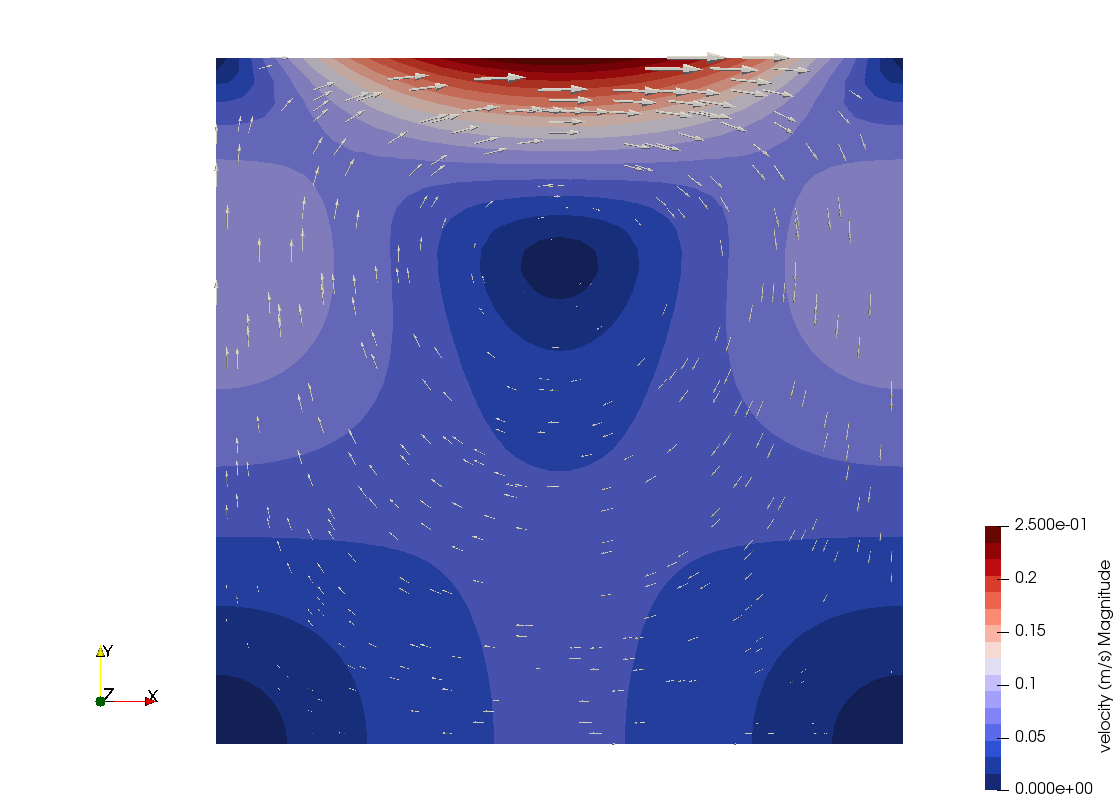
\includegraphics[width=4cm]{python_codes/fieldstone_87/results/experiment_00/vel}
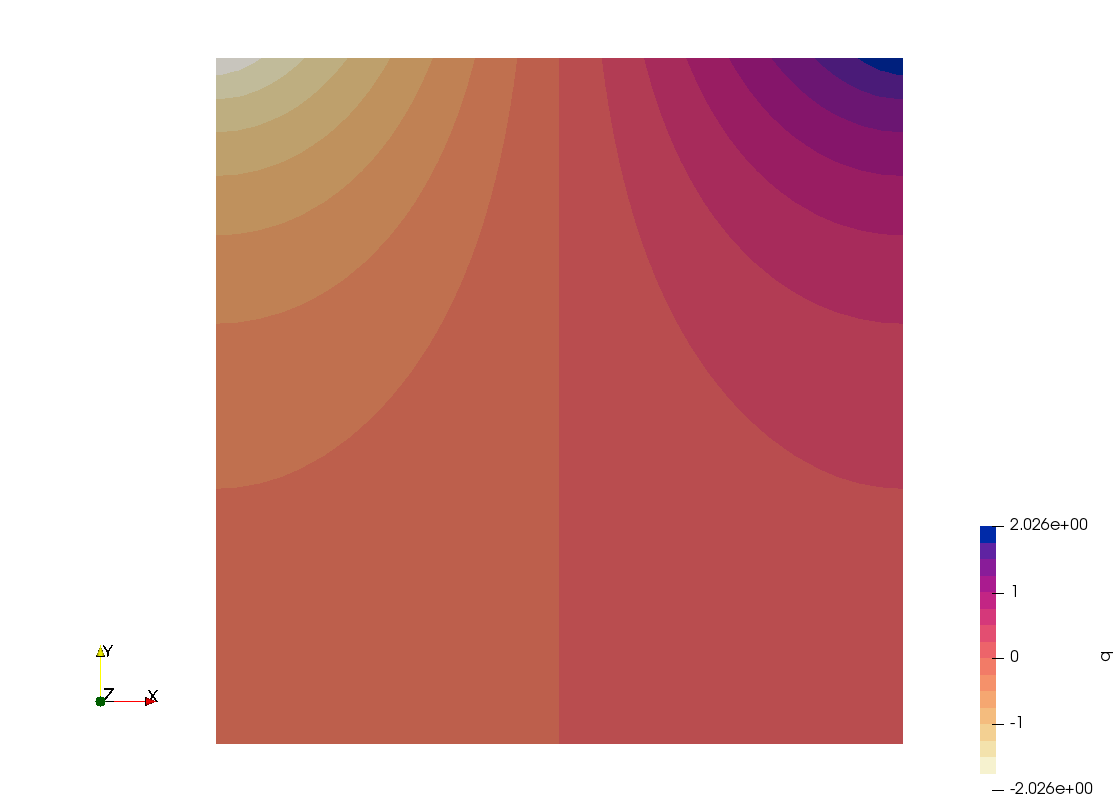
\includegraphics[width=4cm]{python_codes/fieldstone_87/results/experiment_00/p}
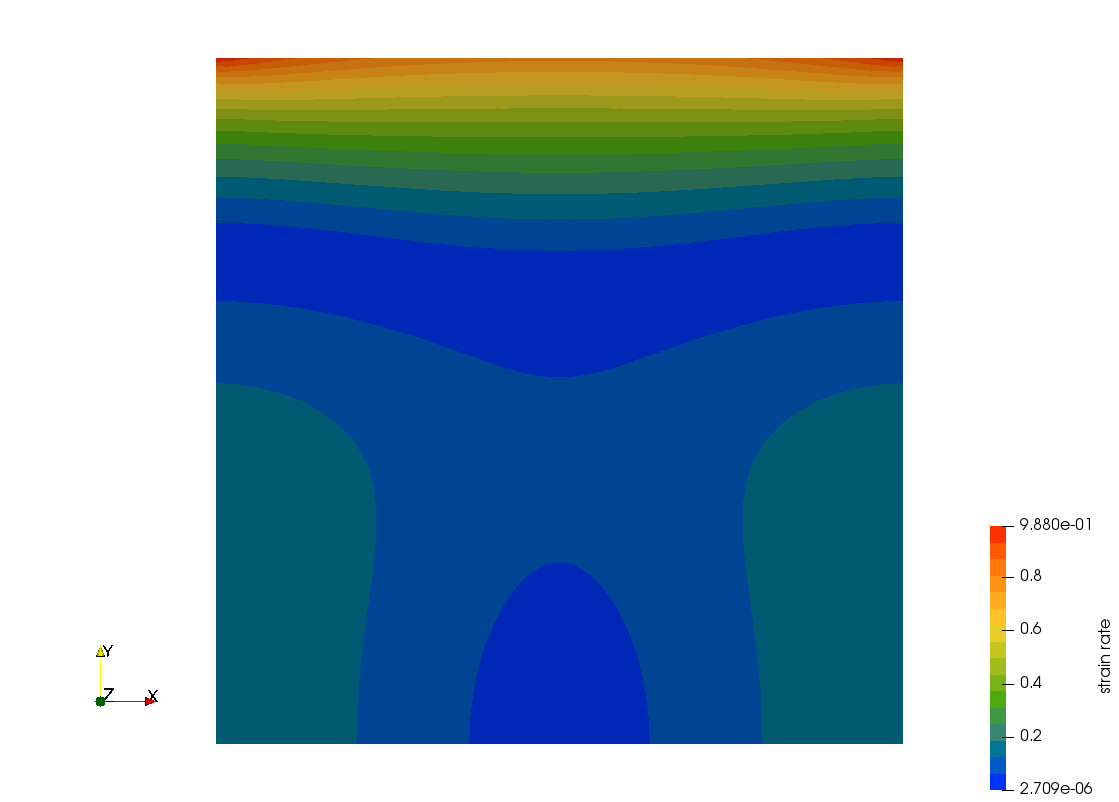
\includegraphics[width=4cm]{python_codes/fieldstone_87/results/experiment_00/sr}\\
{\captionfont Solution as obtained on a $32\times 32$ grid.}
\end{center}

\noindent Four defect correction Picard iterations are carried out and the solution for 
each iteration is shown here under:  

\begin{center}
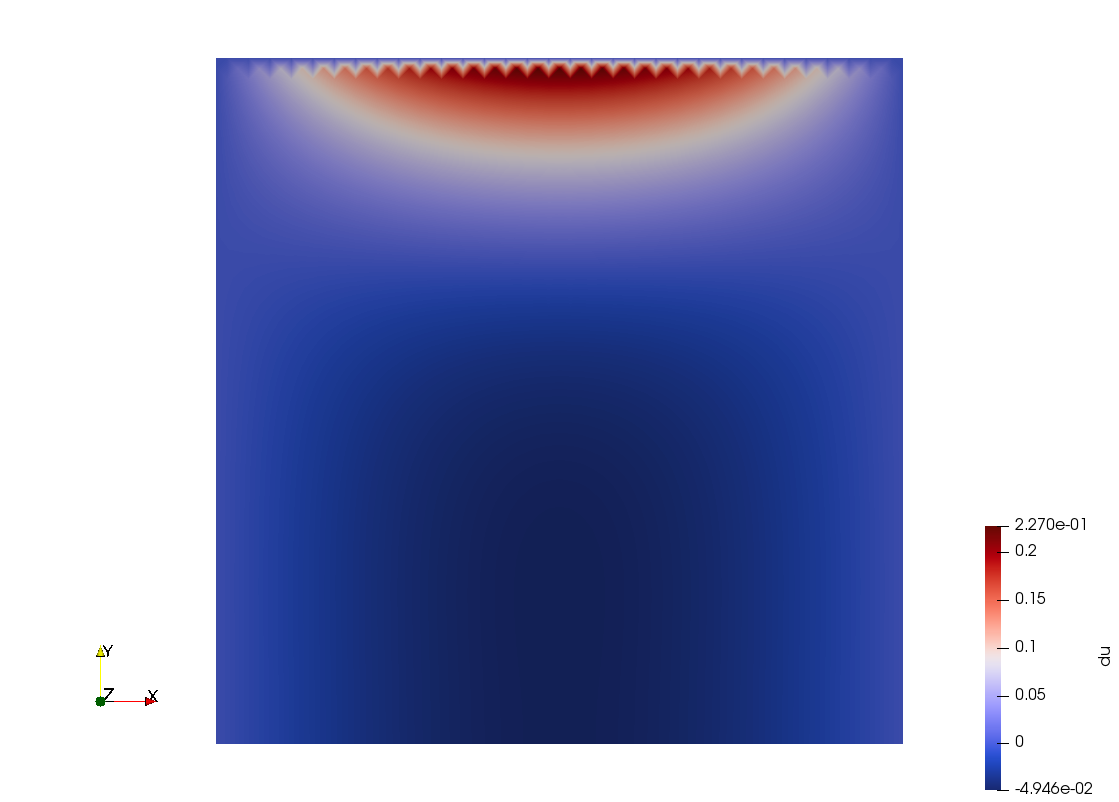
\includegraphics[width=3.4cm]{python_codes/fieldstone_87/results/experiment_00/du_00}
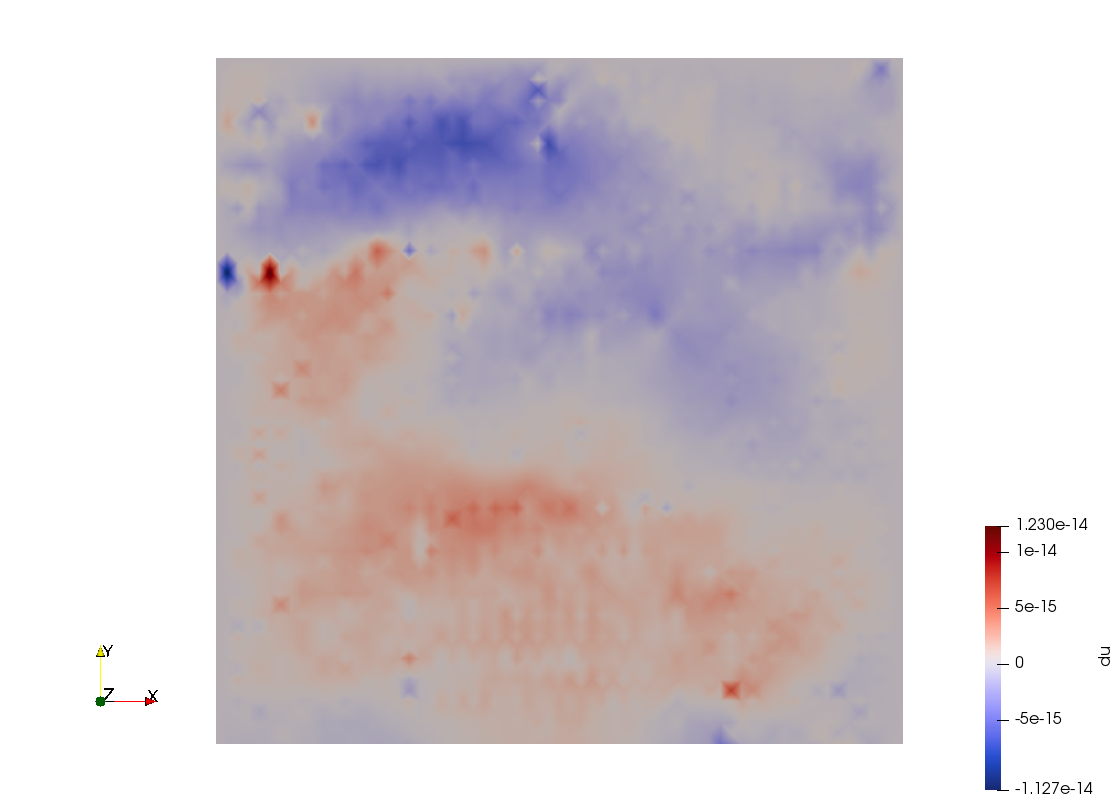
\includegraphics[width=3.4cm]{python_codes/fieldstone_87/results/experiment_00/du_01}
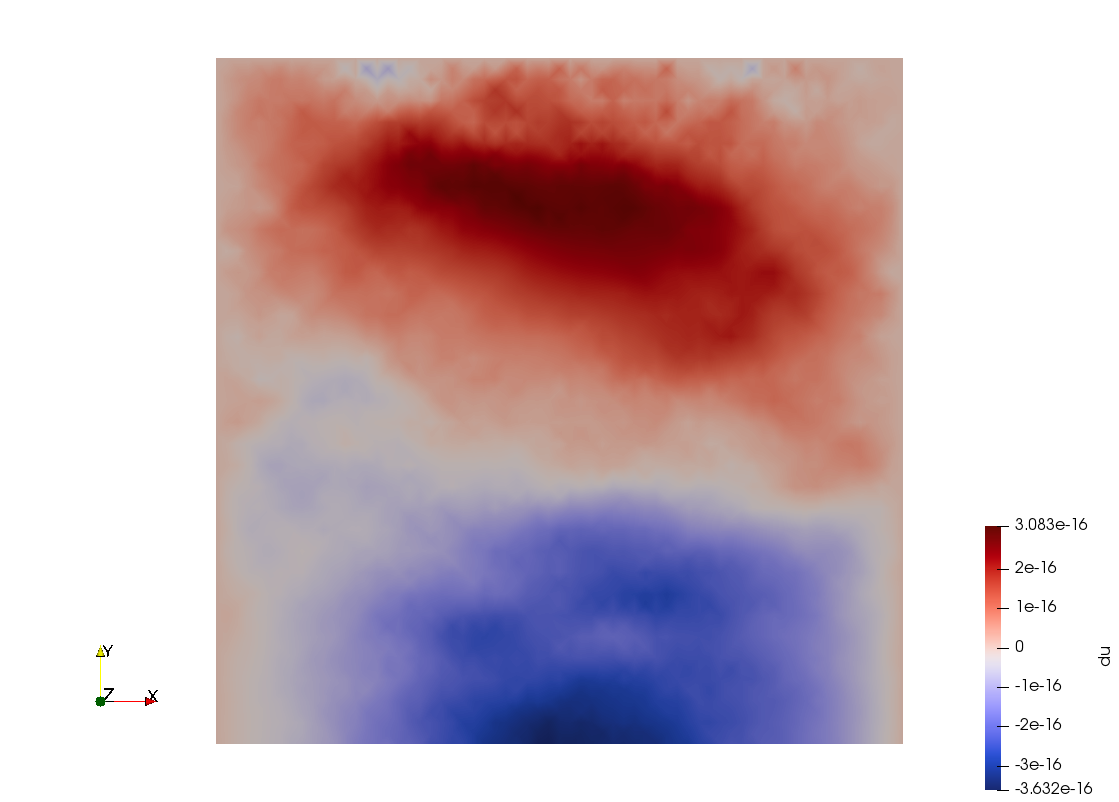
\includegraphics[width=3.4cm]{python_codes/fieldstone_87/results/experiment_00/du_02}
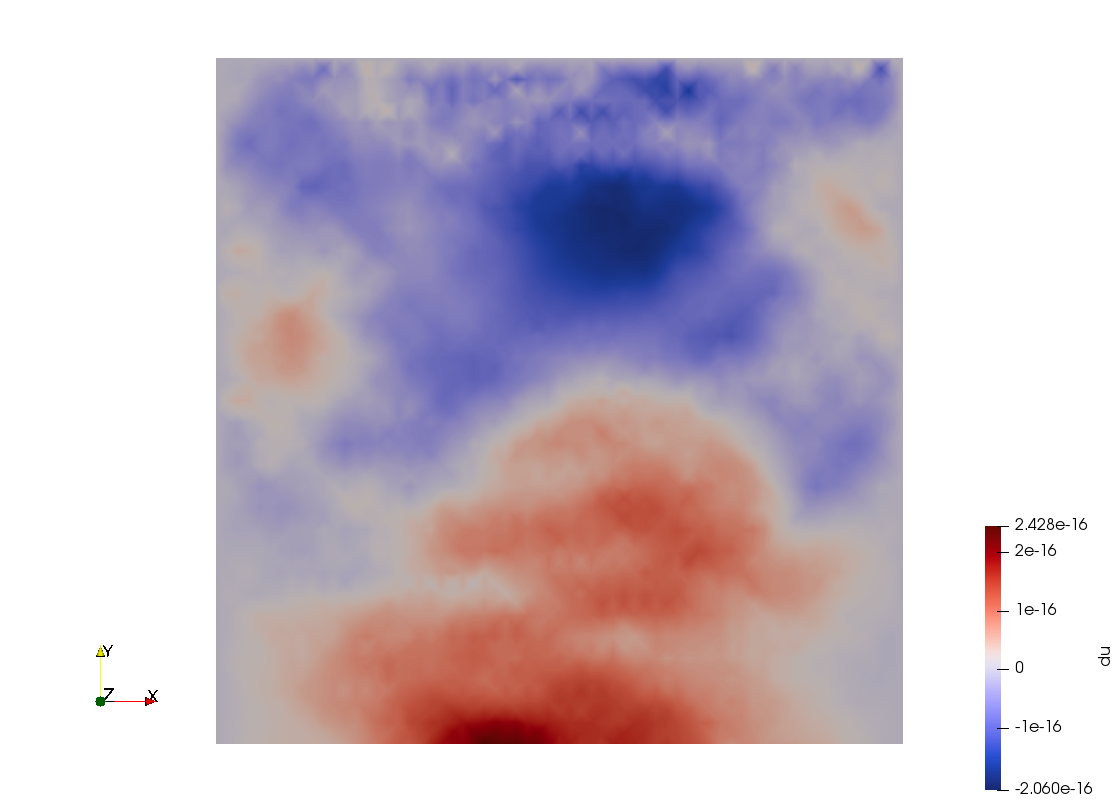
\includegraphics[width=3.4cm]{python_codes/fieldstone_87/results/experiment_00/du_03}\\
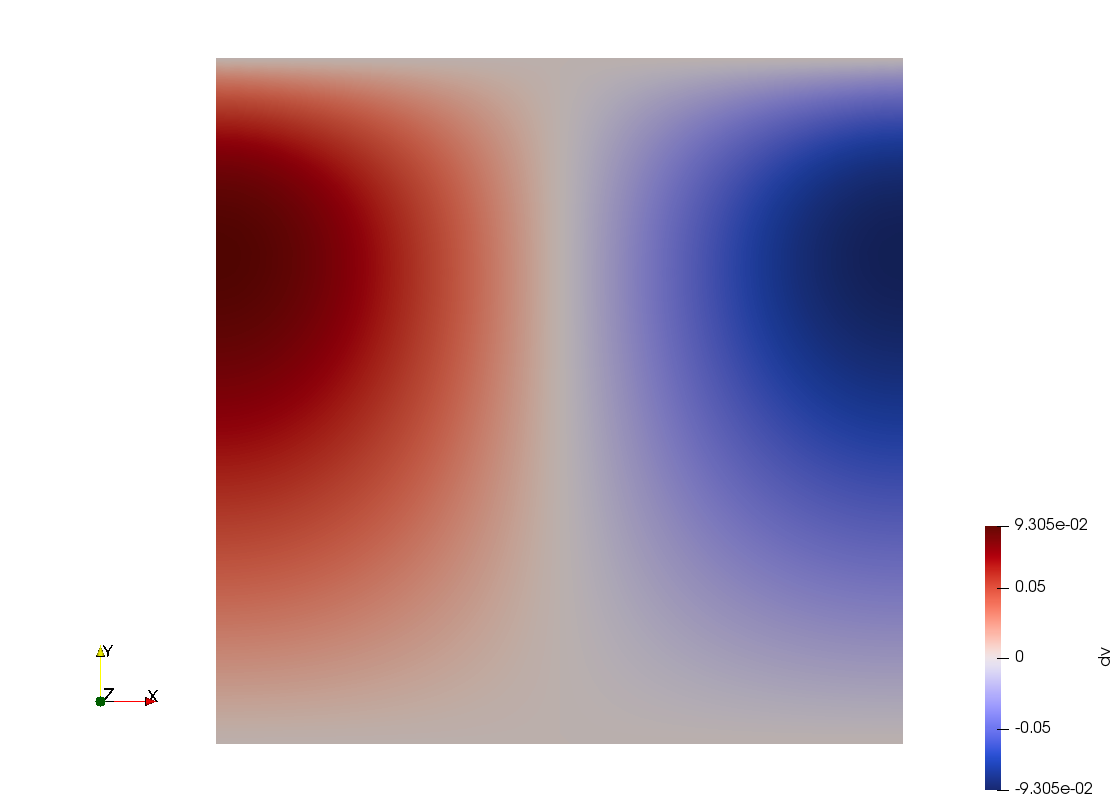
\includegraphics[width=3.4cm]{python_codes/fieldstone_87/results/experiment_00/dv_00}
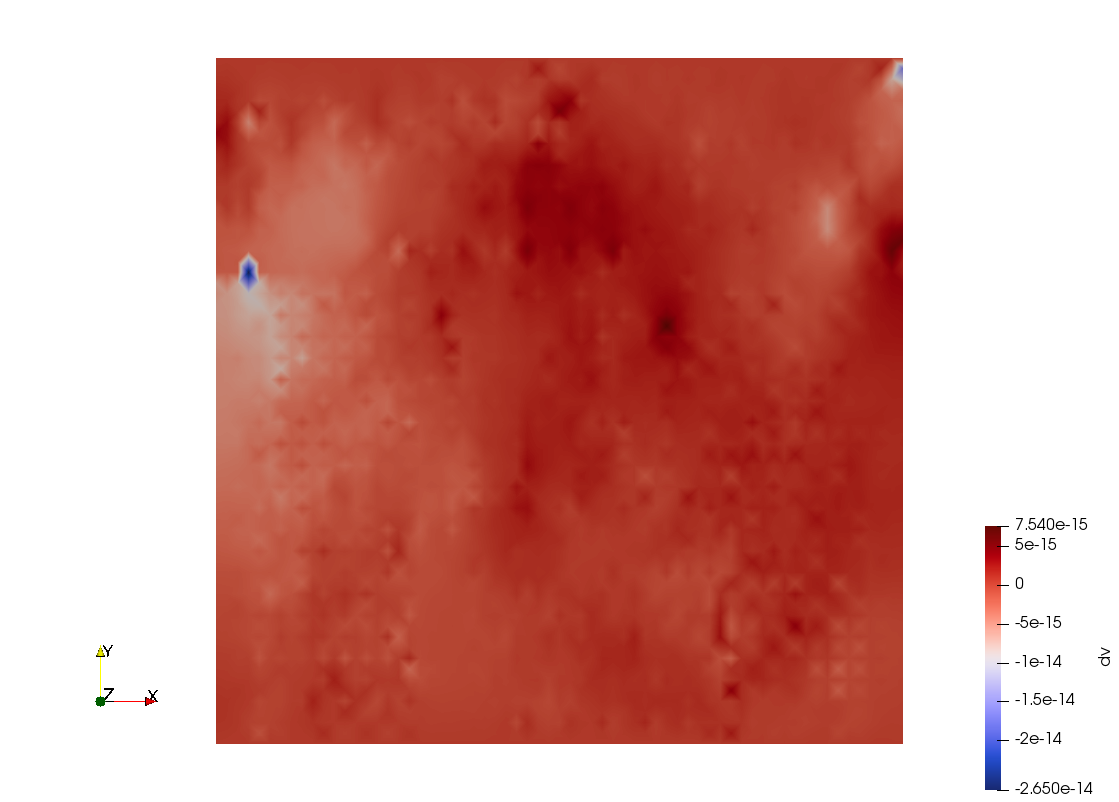
\includegraphics[width=3.4cm]{python_codes/fieldstone_87/results/experiment_00/dv_01}
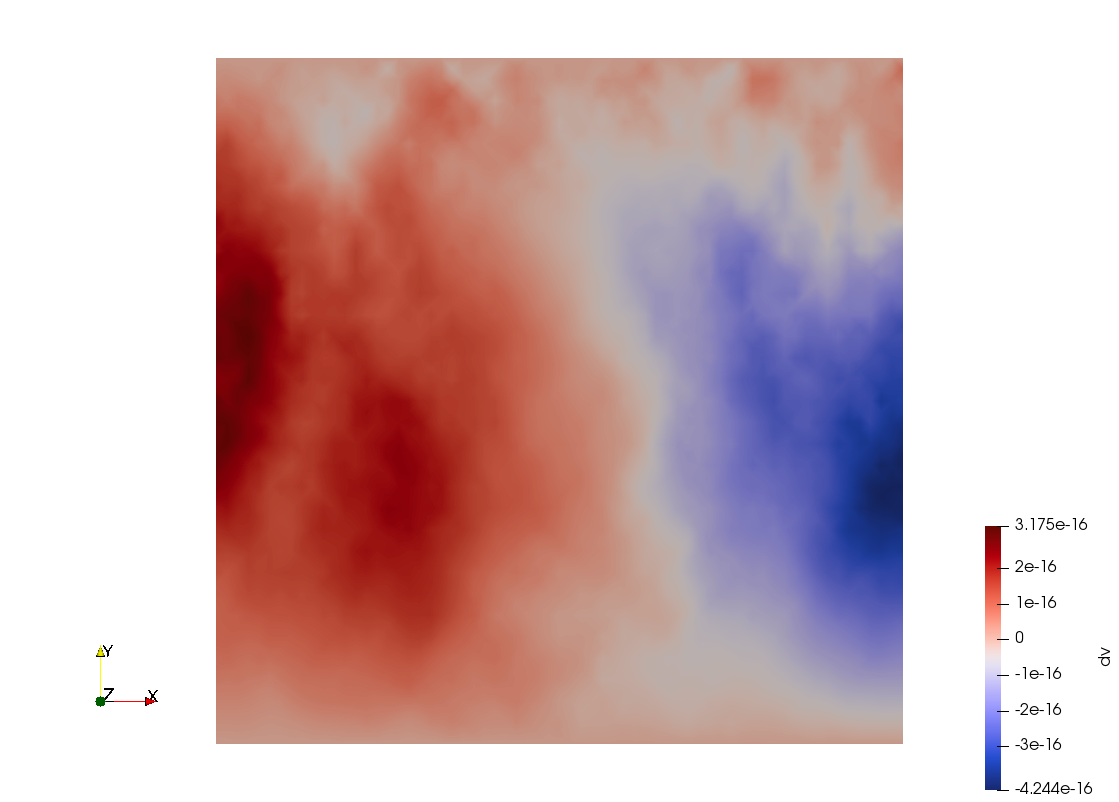
\includegraphics[width=3.4cm]{python_codes/fieldstone_87/results/experiment_00/dv_02}
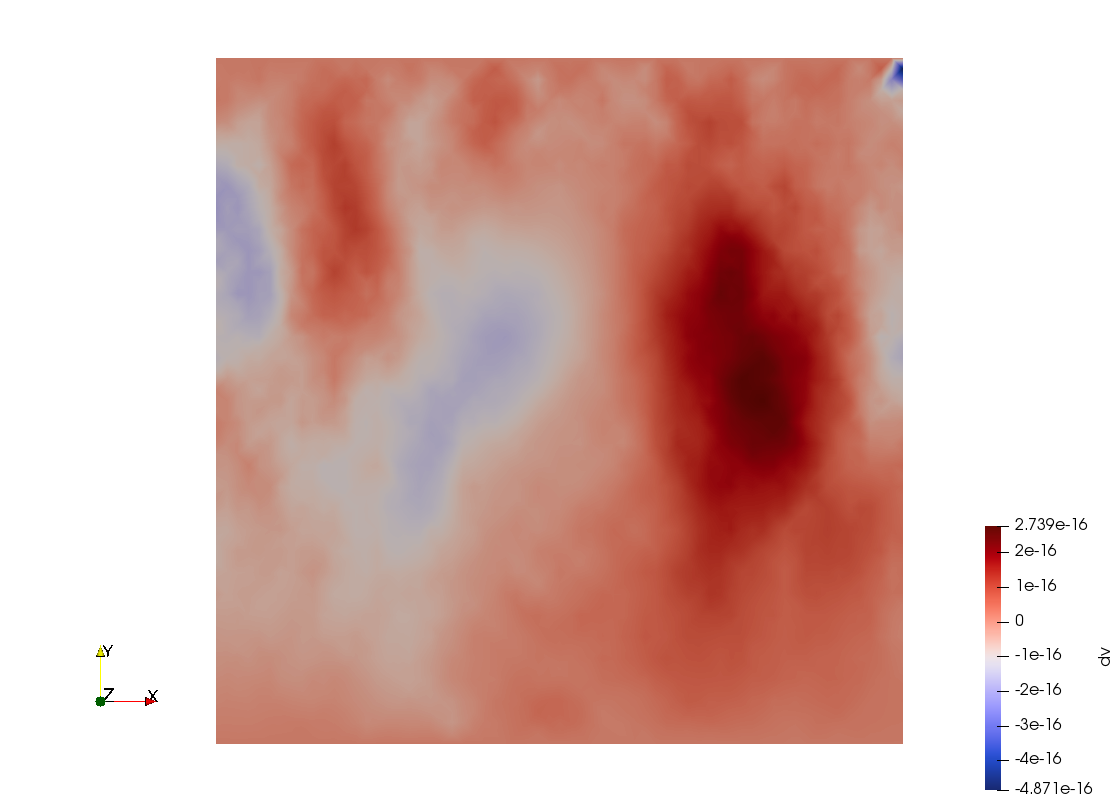
\includegraphics[width=3.4cm]{python_codes/fieldstone_87/results/experiment_00/dv_03}\\
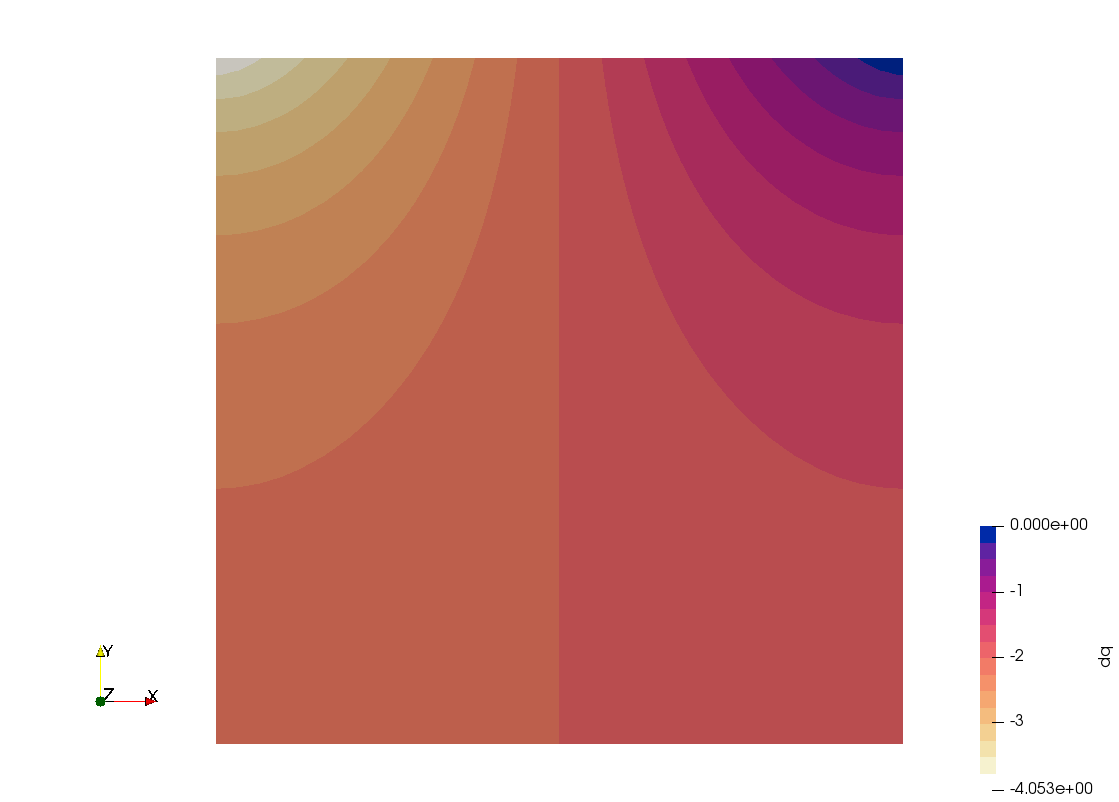
\includegraphics[width=3.4cm]{python_codes/fieldstone_87/results/experiment_00/dp_00}
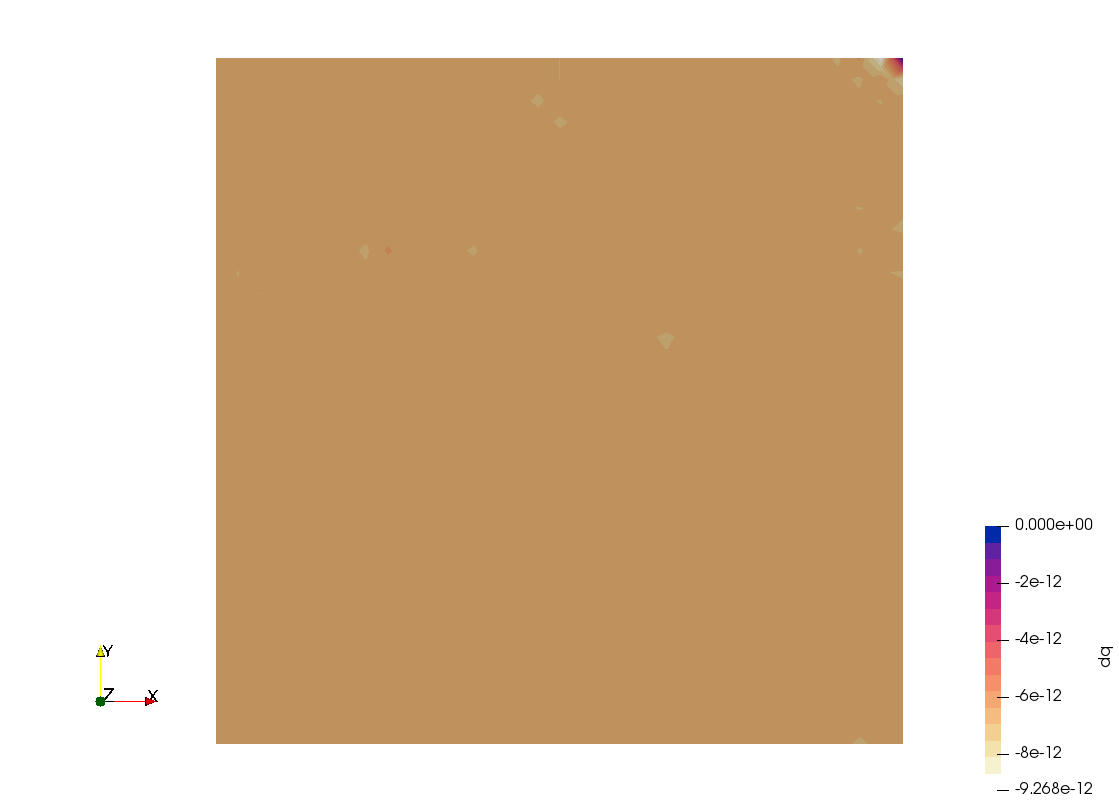
\includegraphics[width=3.4cm]{python_codes/fieldstone_87/results/experiment_00/dp_01}
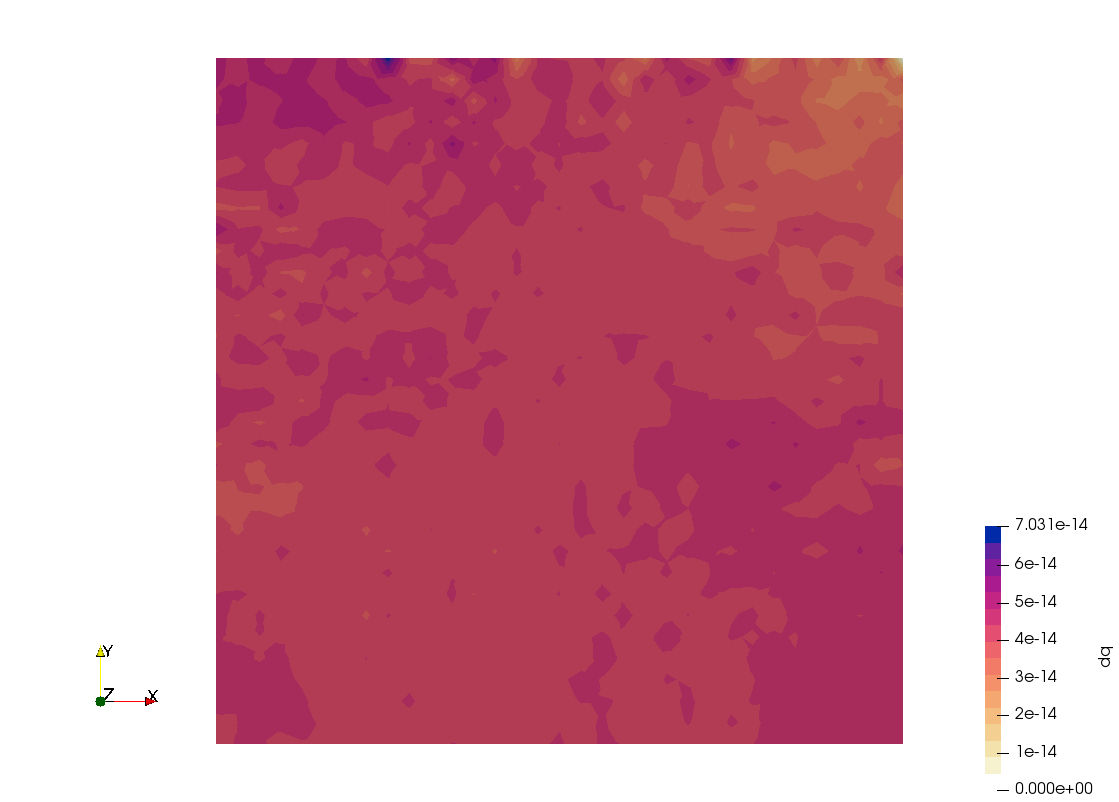
\includegraphics[width=3.4cm]{python_codes/fieldstone_87/results/experiment_00/dp_02}
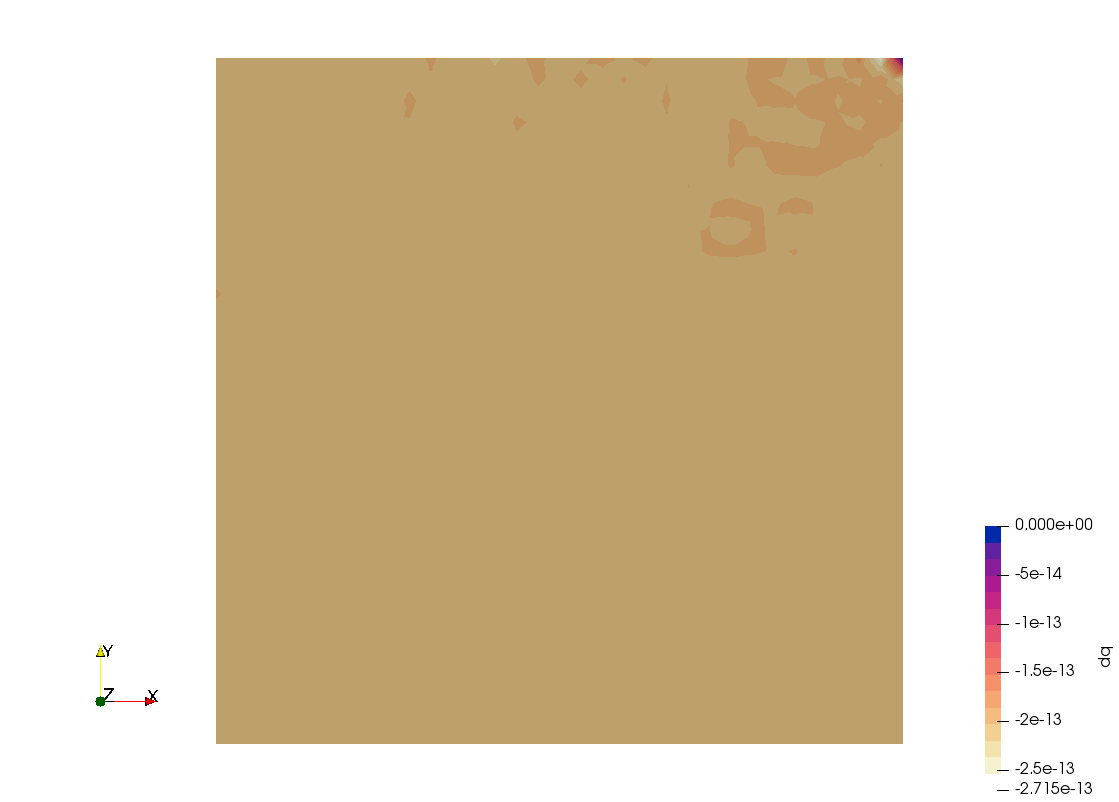
\includegraphics[width=3.4cm]{python_codes/fieldstone_87/results/experiment_00/dp_03}\\
{\captionfont From left to right: iteration 0,1,2,3. 
Top to bottom: horizontali and vertical component of the velocity correction, 
and pressure correction, as obtained on a $32\times 32$ grid. The fields obtained at iteration 0 
are in fact the solution, and all other subsequently obtained fields 
are essentially zero, as expected.}
\end{center}

This is now the same experiment as above but the viscosity is now of the 
power law type with $B=1$ and $n>1$. Also, no-slip boundary conditions 
are prescribed on the left, right and bottom sides. 
The regularisation parameter $\dot{e}$ is set to $10^{-6}$.

\begin{center}
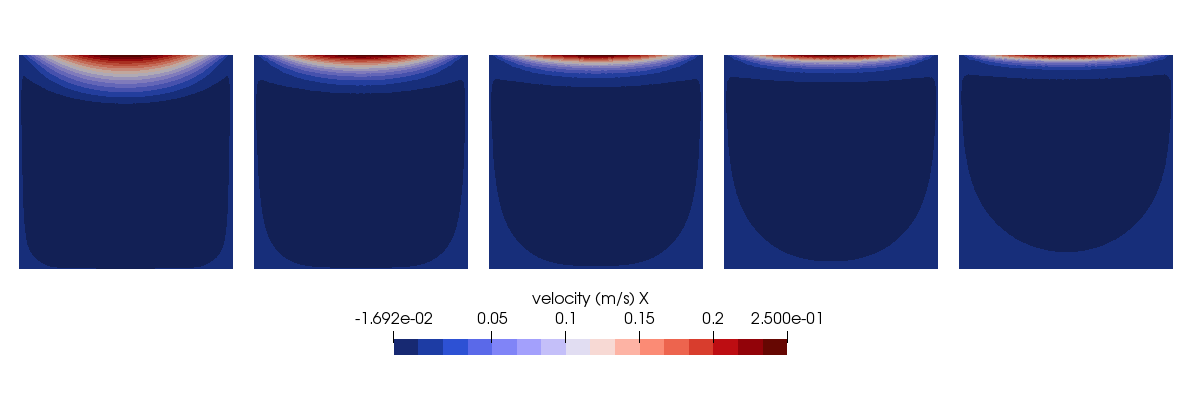
\includegraphics[width=8cm]{python_codes/fieldstone_87/results/experiment_01/meth3/u.png}
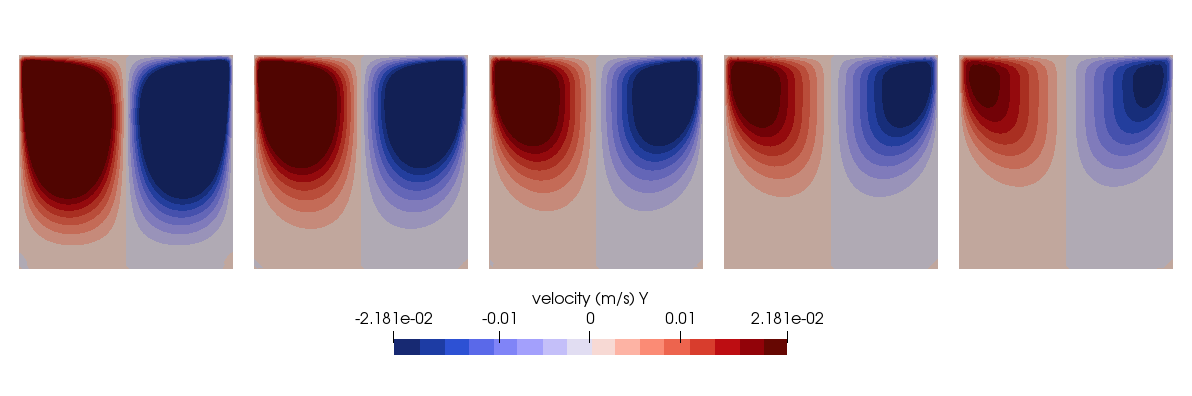
\includegraphics[width=8cm]{python_codes/fieldstone_87/results/experiment_01/meth3/v.png}\\
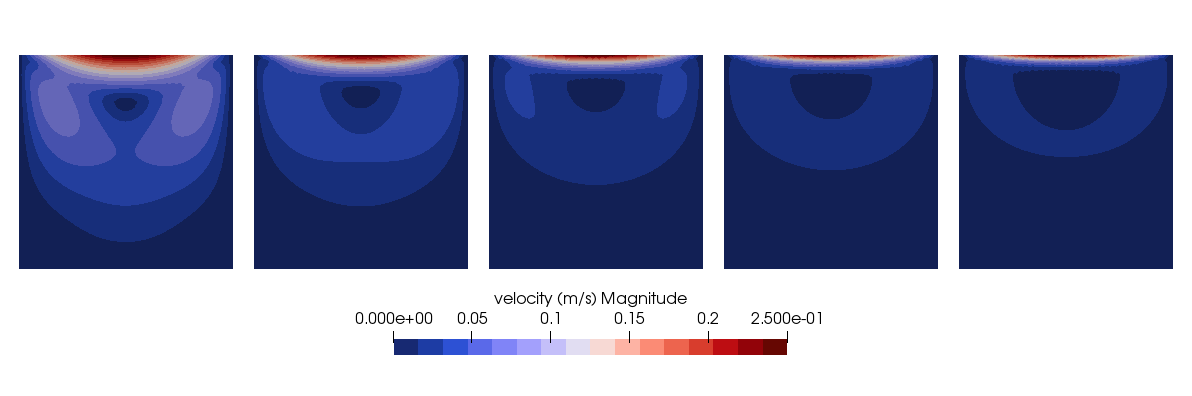
\includegraphics[width=8cm]{python_codes/fieldstone_87/results/experiment_01/meth3/vel.png}
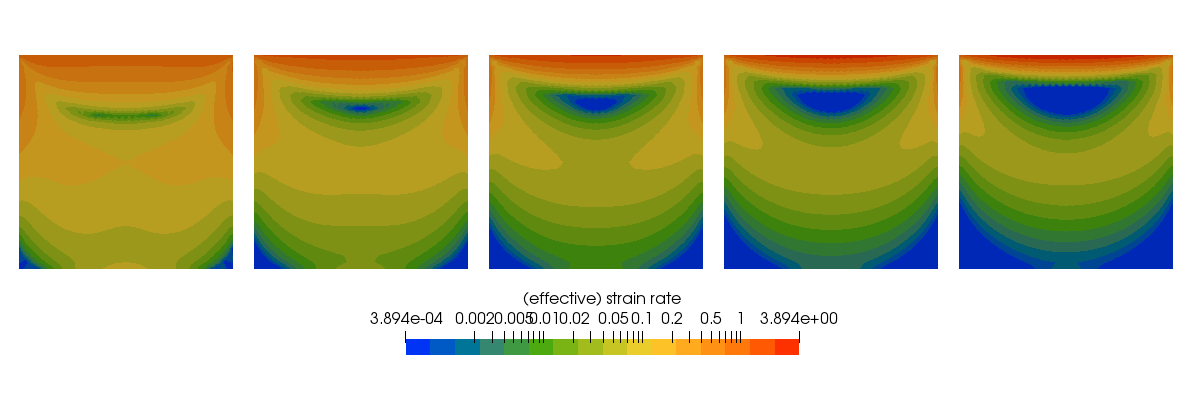
\includegraphics[width=8cm]{python_codes/fieldstone_87/results/experiment_01/meth3/sr.png}\\
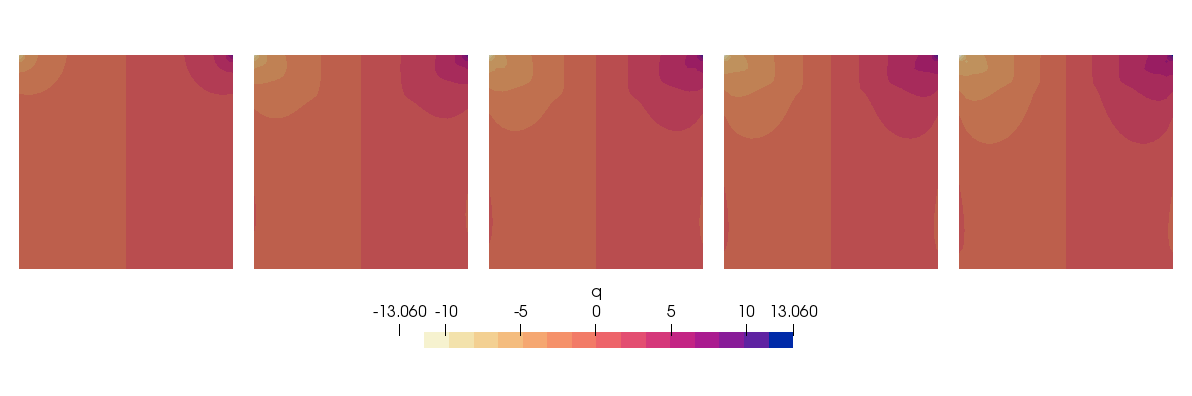
\includegraphics[width=8cm]{python_codes/fieldstone_87/results/experiment_01/meth3/press.png}
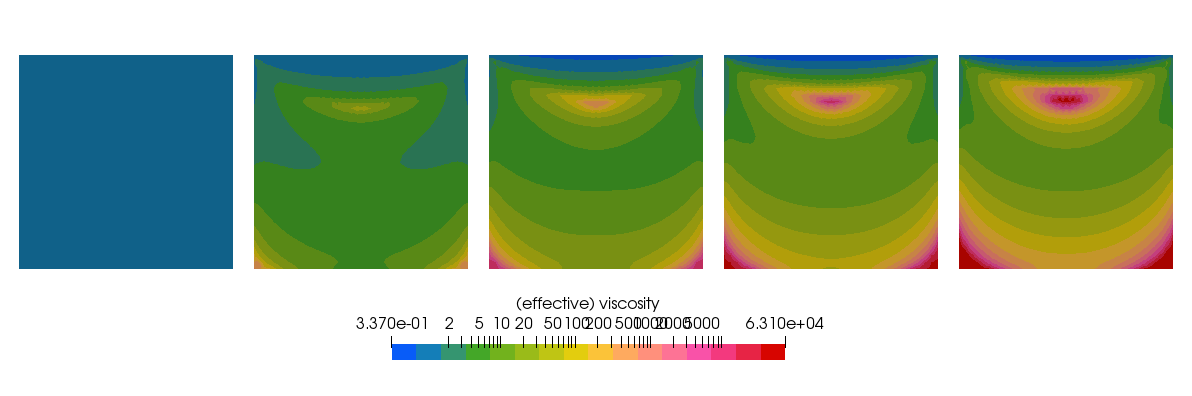
\includegraphics[width=8cm]{python_codes/fieldstone_87/results/experiment_01/meth3/eta.png}\\
{\captionfont Velocity, pressure, strain rate and viscosity fields as a function 
of $n$ (from left to right: 1,2,3,4,5).} 
\end{center}

\begin{center}
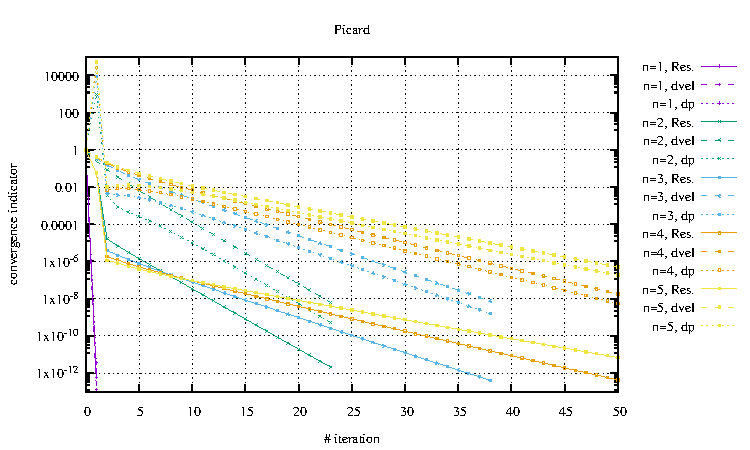
\includegraphics[width=7cm]{python_codes/fieldstone_87/results/experiment_01/conv_picard.pdf}
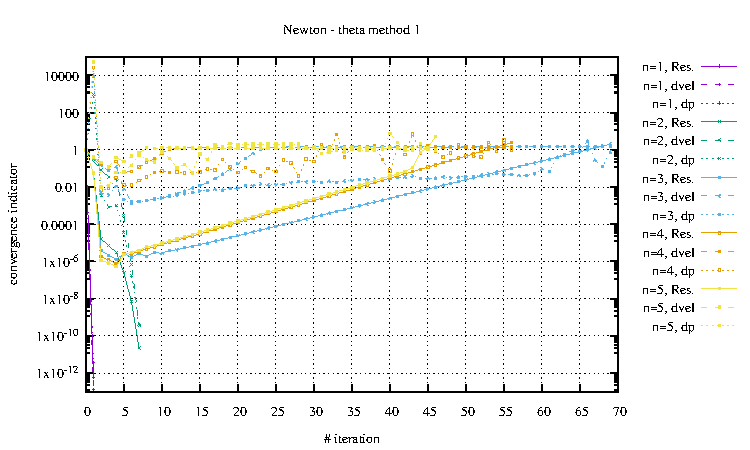
\includegraphics[width=7cm]{python_codes/fieldstone_87/results/experiment_01/conv_meth1.pdf}\\
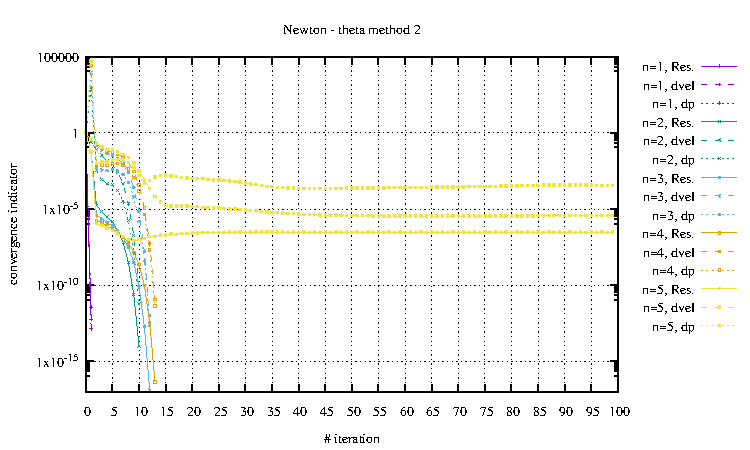
\includegraphics[width=7cm]{python_codes/fieldstone_87/results/experiment_01/conv_meth2.pdf}
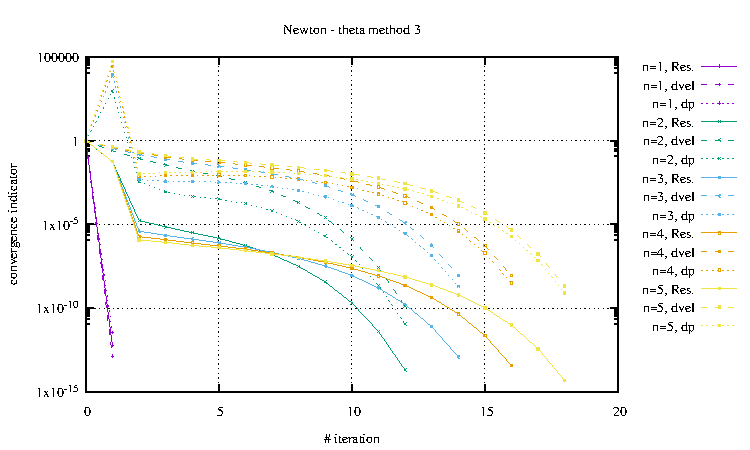
\includegraphics[width=7cm]{python_codes/fieldstone_87/results/experiment_01/conv_meth3.pdf}\\
{\captionfont Npicard =4. $\dot{e}=10^{-6}$}
\end{center}


\begin{center}
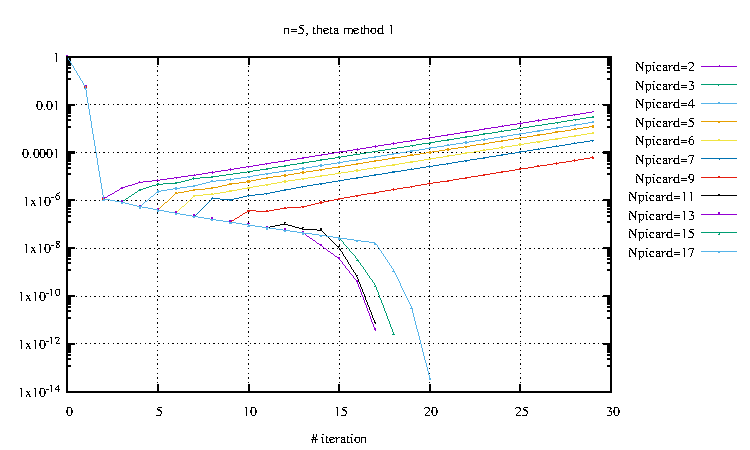
\includegraphics[width=5.7cm]{python_codes/fieldstone_87/results/experiment_01/conv_n5_meth1}
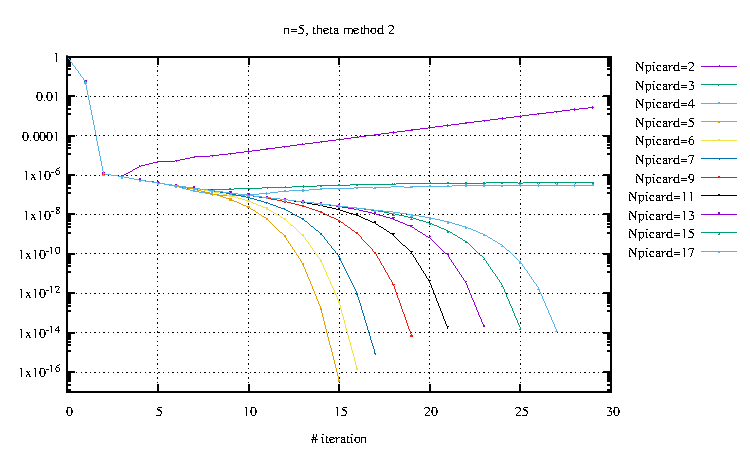
\includegraphics[width=5.7cm]{python_codes/fieldstone_87/results/experiment_01/conv_n5_meth2}
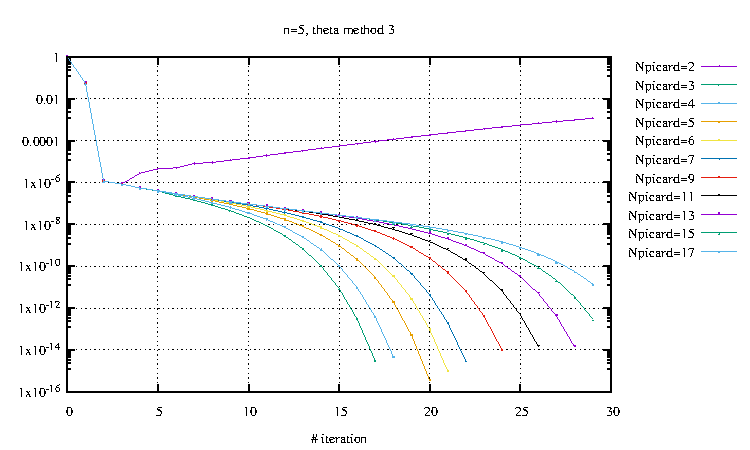
\includegraphics[width=5.7cm]{python_codes/fieldstone_87/results/experiment_01/conv_n5_meth3}\\
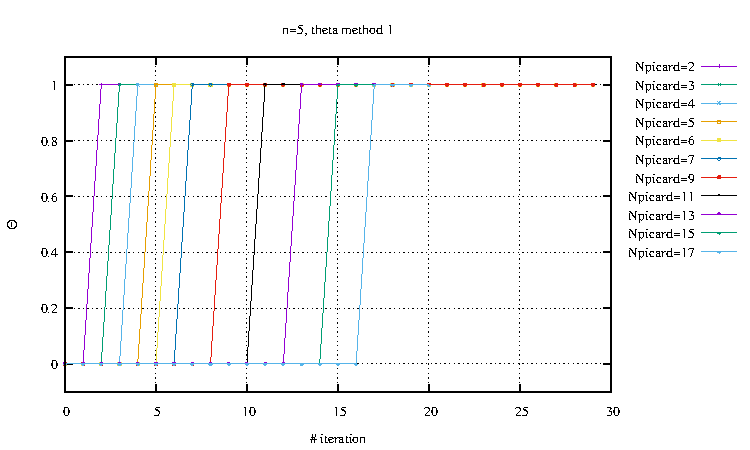
\includegraphics[width=5.7cm]{python_codes/fieldstone_87/results/experiment_01/theta_n5_meth1}
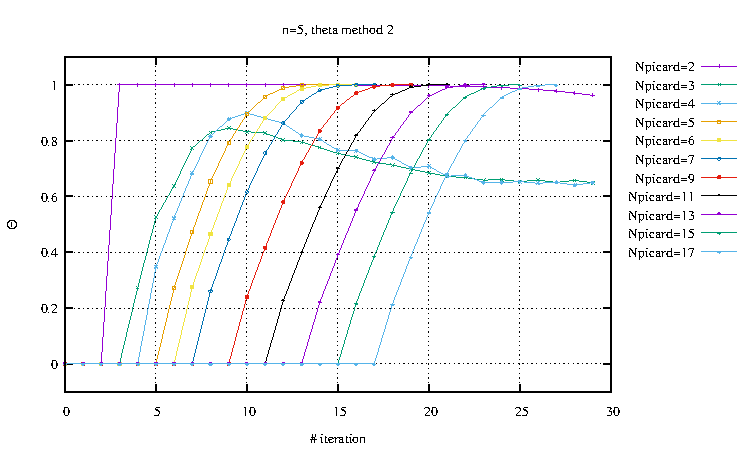
\includegraphics[width=5.7cm]{python_codes/fieldstone_87/results/experiment_01/theta_n5_meth2}
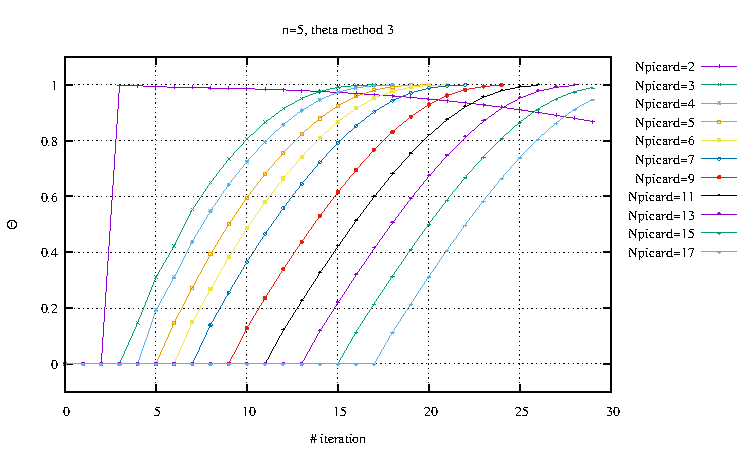
\includegraphics[width=5.7cm]{python_codes/fieldstone_87/results/experiment_01/theta_n5_meth3}\\
{\captionfont Influence of the number of Picard iterations before wtiching to Newton ones for $n=5$.}
\end{center}


\begin{center}
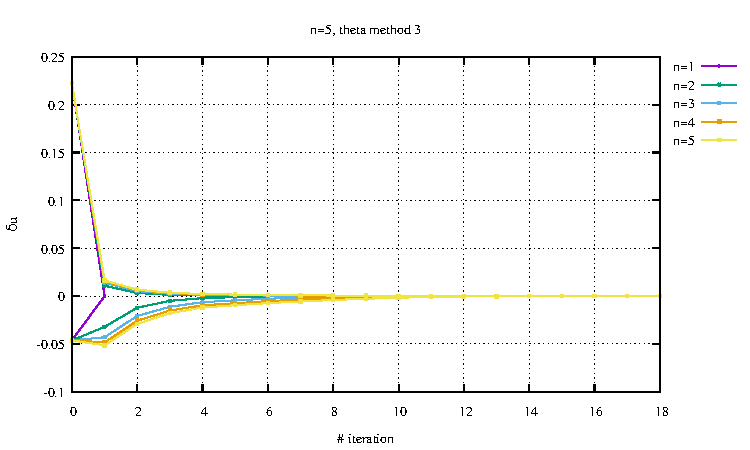
\includegraphics[width=5.7cm]{python_codes/fieldstone_87/results/experiment_01/du_meth3.pdf}
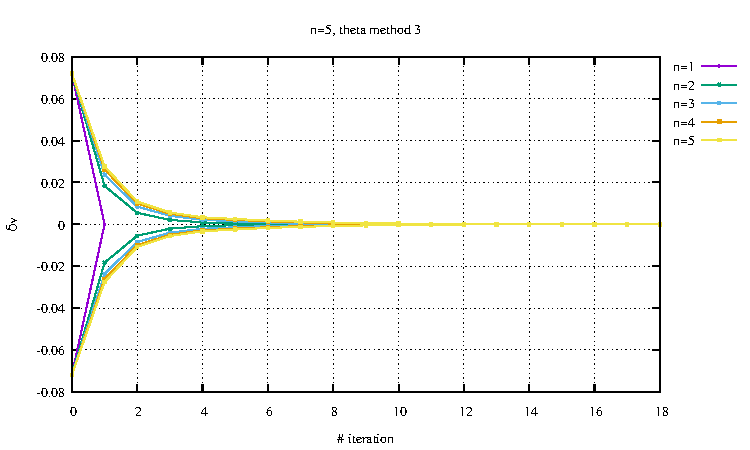
\includegraphics[width=5.7cm]{python_codes/fieldstone_87/results/experiment_01/dv_meth3.pdf}
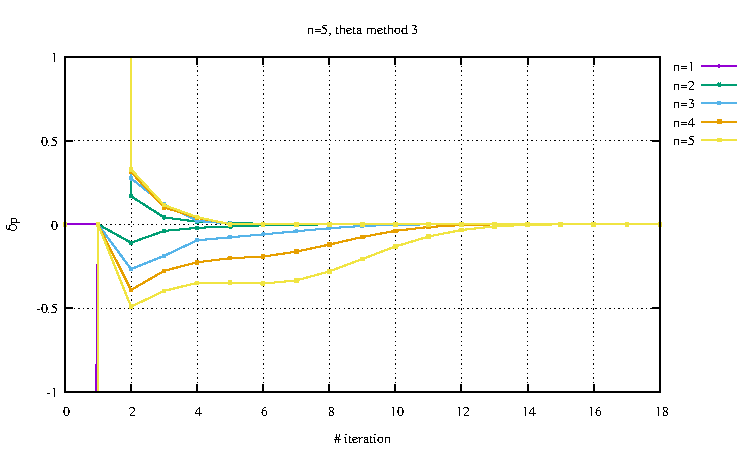
\includegraphics[width=5.7cm]{python_codes/fieldstone_87/results/experiment_01/dp_meth3.pdf}\\
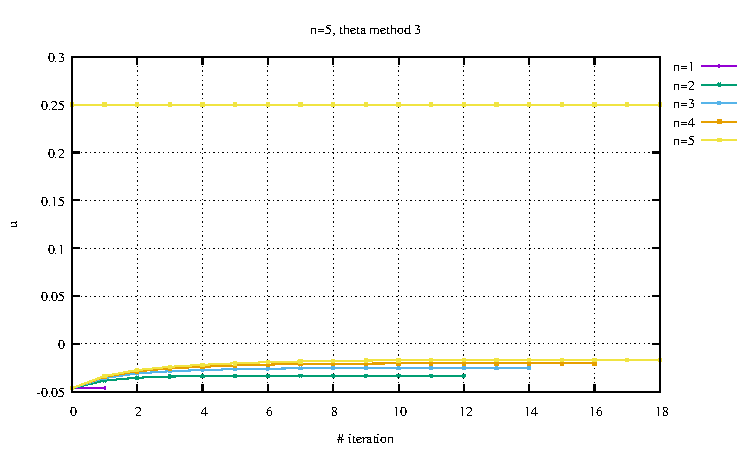
\includegraphics[width=5.7cm]{python_codes/fieldstone_87/results/experiment_01/u_meth3.pdf}
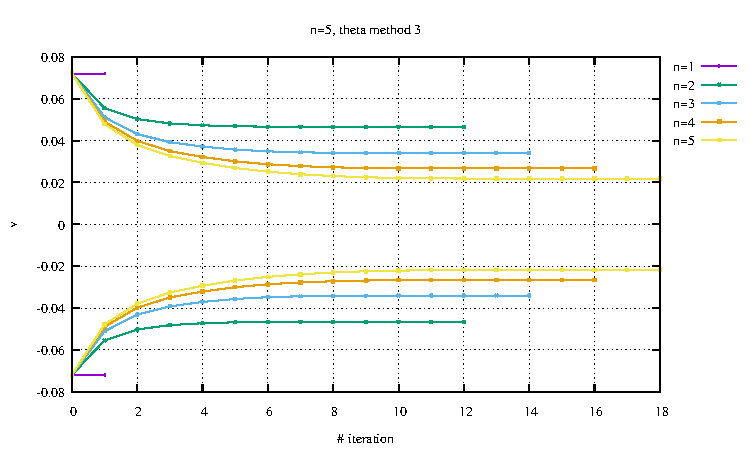
\includegraphics[width=5.7cm]{python_codes/fieldstone_87/results/experiment_01/v_meth3.pdf}
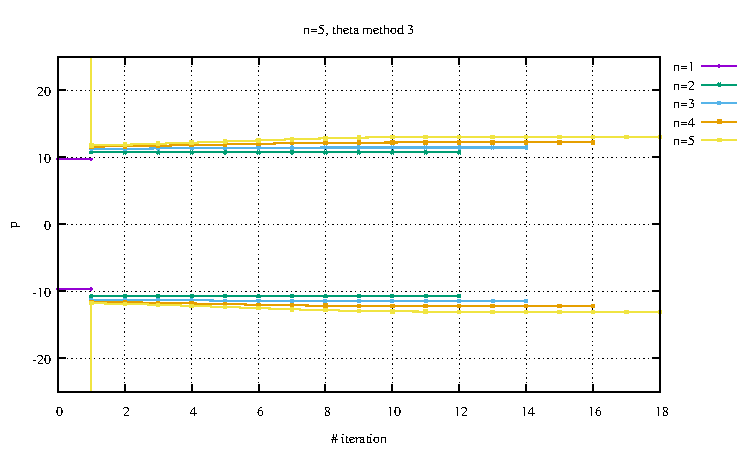
\includegraphics[width=5.7cm]{python_codes/fieldstone_87/results/experiment_01/p_meth3.pdf}
\end{center}




\newpage
%--------------------------------------------------------------------------
\subsubsection*{Experiment 2 - the brick }

Following Christensen (1992) \cite{chri92} and Ciskova et al (2002) \cite{civv02} 
one can use the following relationship to include a form of plasticity through stress limiting:
\[
\frac{\tau}{\tau_{lim}} = \left( \frac{ \dot{\varepsilon}_e  }{ \dot{\varepsilon}_{lim}  }  \right)^{1/n}
\]
where $\tau_{lim}$ is the yield stress and $n$ is the power-law index defining the 'brittleness'
of the material. In Ciskova et al. (2002), 
the authors use $n=5$, $\dot{\varepsilon}_{lim}=10^{-15}\si{\per\second}$, 
and $\tau_{lim}=10^{9}\si{\pascal}$. 

In this experiment the domain is 40x10\si{\kilo\metre} and the resolution is $64\times 16$ elements. 
The regularisation parameter is set to $\dot{e}=10^{-20}\si{\per\second}$.
Because we here consider a shallow upper-crustal 
layer, the material is characterised by a cohesion of $c=40\si{\mega\pascal}=\tau_{lim}$.
Extensional boundary conditions are applied so that the background strain rate is 
also $10^{-15}\si{\per\second}$.

One can also look at the effective viscosity by 
setting $\tau = 2 \eta_{eff} \dot{\varepsilon}_e$ so that
\[
\frac{2 \eta_{eff}\dot{\varepsilon}_e }{\tau_{lim}} = 
\left( \frac{ \dot{\varepsilon}_e  }{ \dot{\varepsilon}_{lim}  }  \right)^{1/n}
\]
which yields
\[
\eta_{eff} = \left( \frac{ \dot{\varepsilon}_e  }{ \dot{\varepsilon}_{lim} } \right)^{1/n}   
\frac{1}{ 2\dot{\varepsilon}_e} \tau_{lim}
=
\left( \frac{ \dot{\varepsilon}_e  }{ \dot{\varepsilon}_{lim}  }  \right)^{1/n} 
\frac{\dot{\varepsilon}_{lim} }{\dot{\varepsilon}_e} \frac{\tau_{lim}   }{2 \dot{\varepsilon}_{lim}} 
=
\left( \frac{ \dot{\varepsilon}_e  }{ \dot{\varepsilon}_{lim}  }  \right)^{\frac{1}{n}-1}  
\frac{\tau_{lim}   }{2 \dot{\varepsilon}_{lim}} 
\]
Defining $\eta_{lim}=\tau_{lim} /  2 \dot{\varepsilon}_{lim}$, then
\[
\eta_{eff} = \eta_{lim} \left( \frac{ \dot{\varepsilon}_e  }{ \dot{\varepsilon}_{lim}  }  
\right)^{\alpha}
\]
In our case, $\eta_{lim}= 4\time 10^7/2/10^{-15}=2\times10^{22}$. 
In the present context, we then define
\[
B
%= \frac{c}{2 \dot{\varepsilon}_{lim}} \frac{1}{\dot{\varepsilon}_{lim}^{\alpha}}
= \frac{ \eta_{lim} }{\dot{\varepsilon}_{lim}^{\alpha}}
\]
and finally 
\[
\eta_{eff} = B \dot{\varepsilon}_e^\alpha \rightarrow B (\dot{\varepsilon}_e^2 + \dot{e}^2 )^{\alpha/2}
\]
Boundary conditions are as follows: $\vec{\upnu}=(-u_{bc},0)$ is imposed on the left and the left half 
of the bottom side, and $\vec{\upnu}=(+u_{bc},0)$ is imposed on the right and the right half
of the bottom side. The top is left free.  

\begin{center}
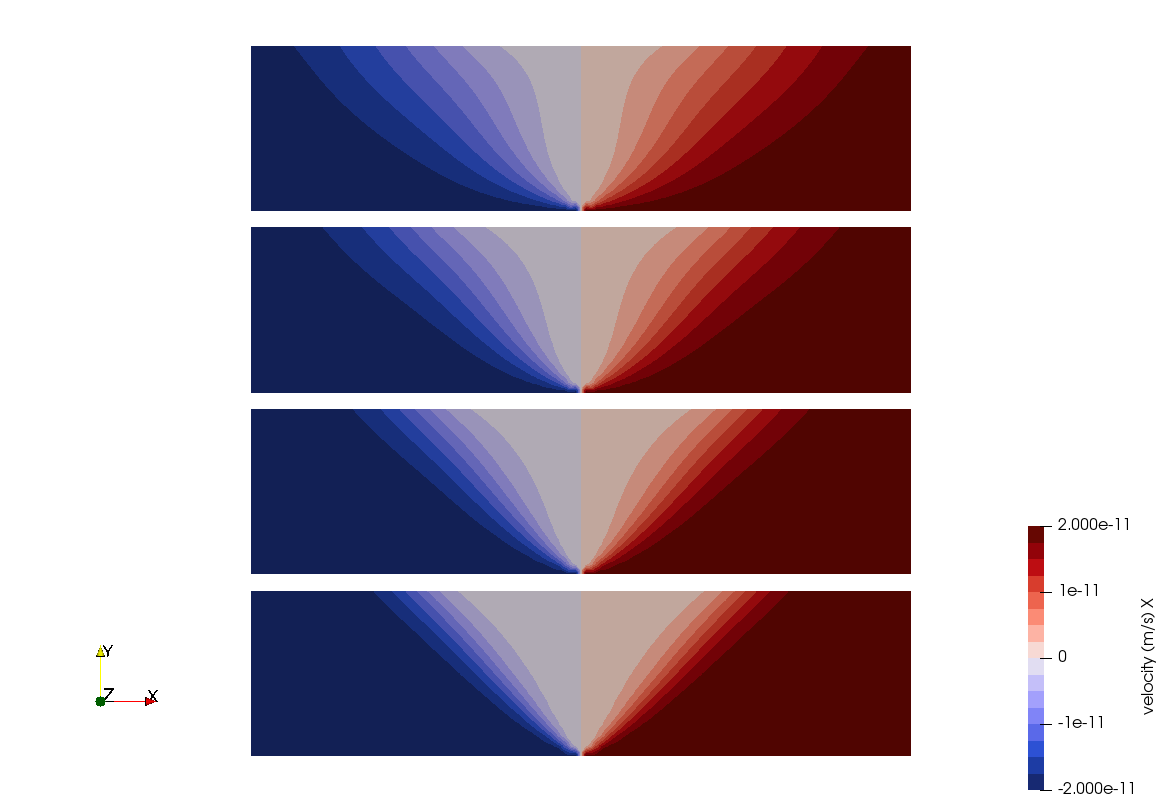
\includegraphics[width=7.5cm]{python_codes/fieldstone_87/results/experiment_02/vel.png}
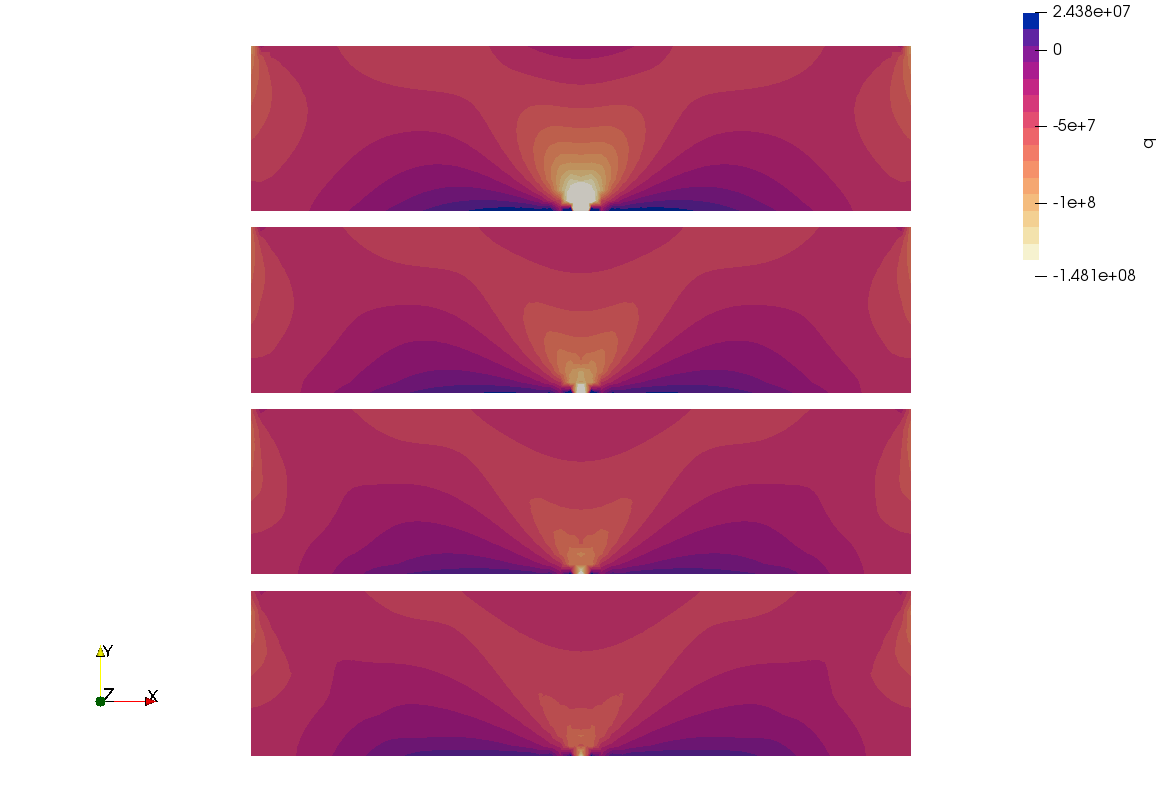
\includegraphics[width=7.5cm]{python_codes/fieldstone_87/results/experiment_02/p.png}\\
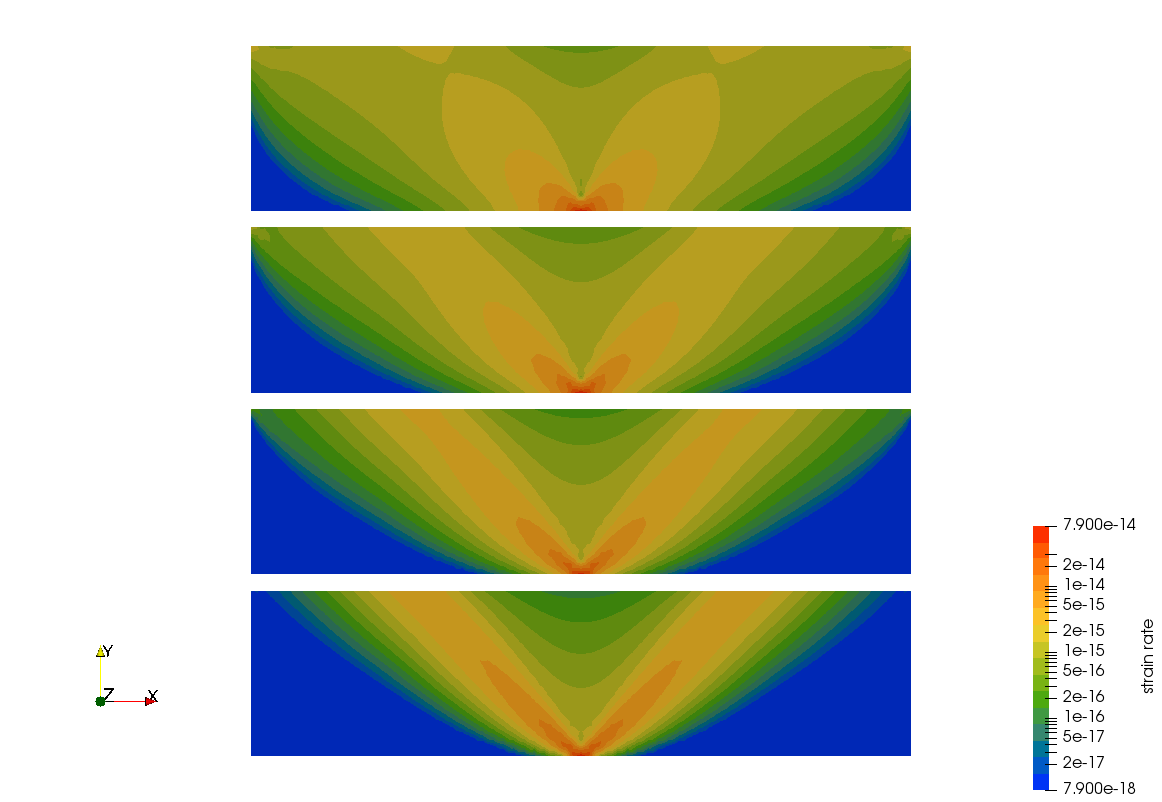
\includegraphics[width=7.5cm]{python_codes/fieldstone_87/results/experiment_02/sr.png}
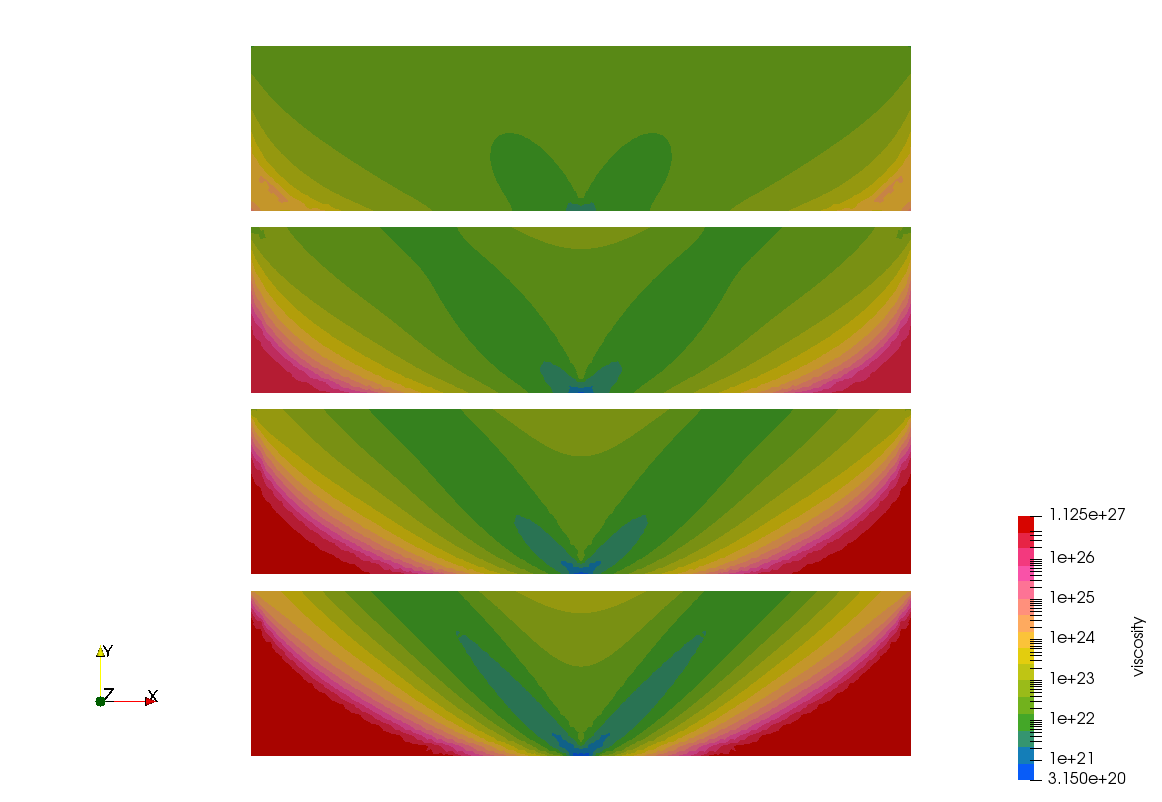
\includegraphics[width=7.5cm]{python_codes/fieldstone_87/results/experiment_02/eta.png}\\
{\captionfont Velocity, pressure, strain rate and viscosity fields as a function 
of $n$ (from top to bottom: 2,5,10,20).} 
\end{center}

\begin{center}
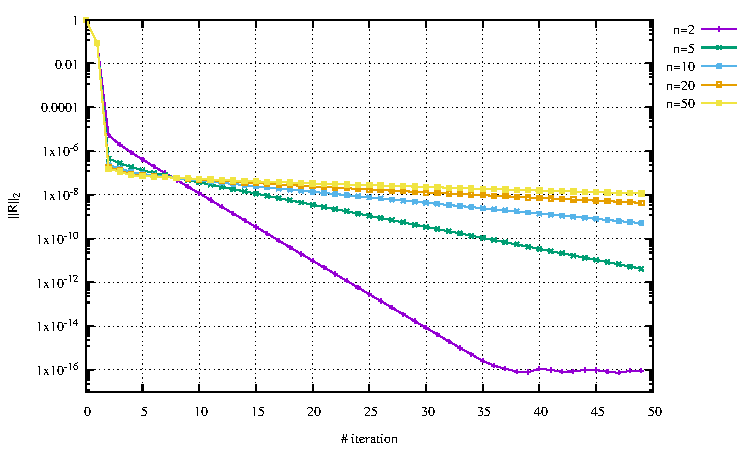
\includegraphics[width=7cm]{python_codes/fieldstone_87/results/experiment_02/conv}
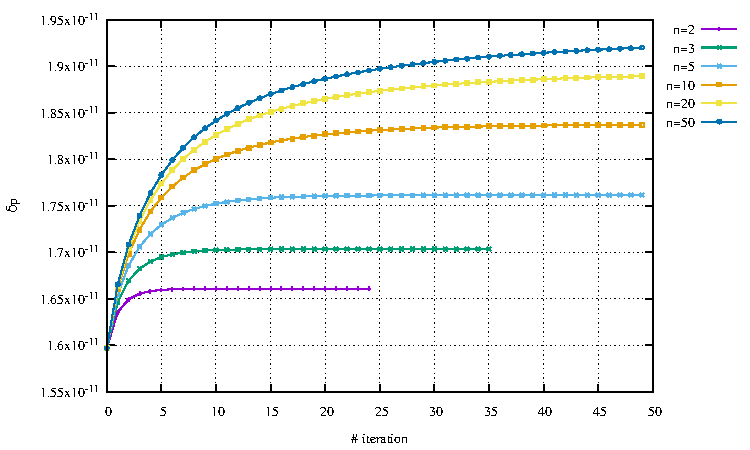
\includegraphics[width=7cm]{python_codes/fieldstone_87/results/experiment_02/vrms}\\
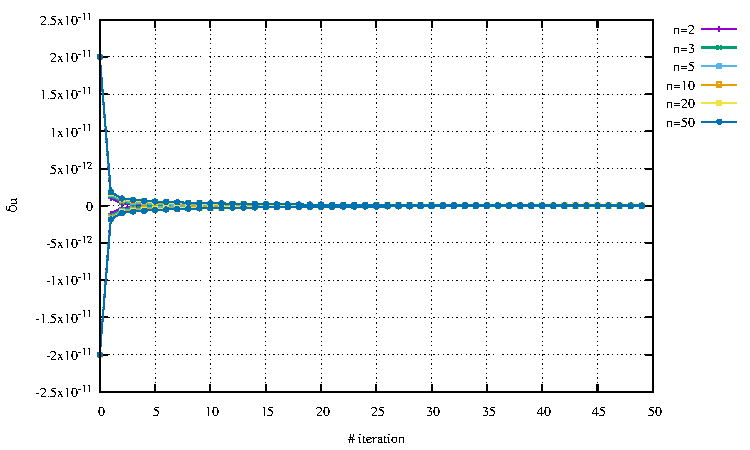
\includegraphics[width=5.7cm]{python_codes/fieldstone_87/results/experiment_02/du}
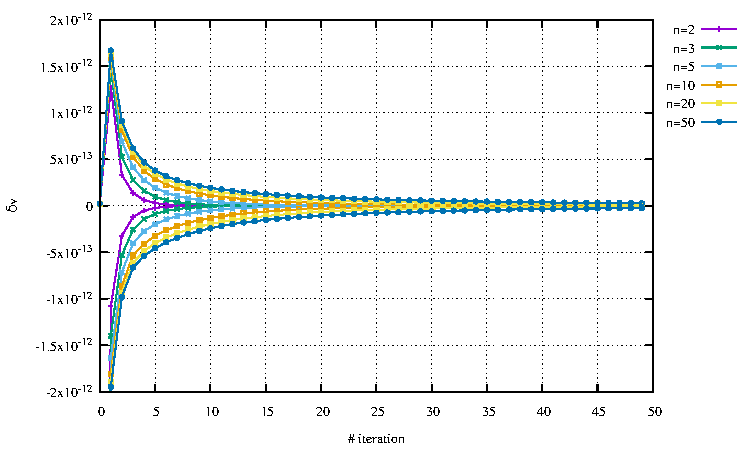
\includegraphics[width=5.7cm]{python_codes/fieldstone_87/results/experiment_02/dv}
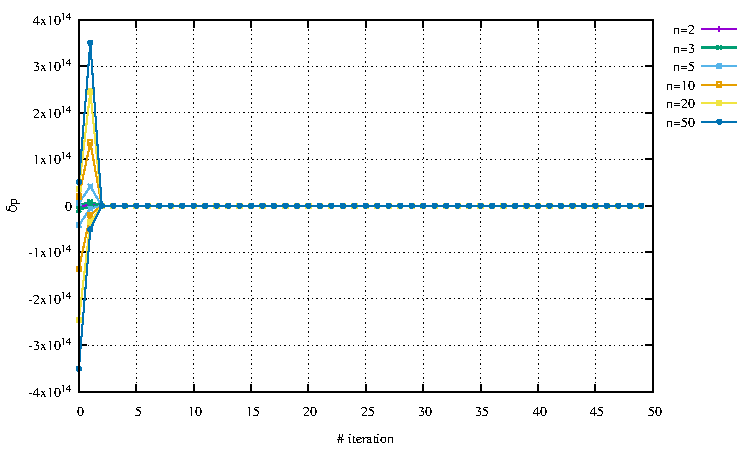
\includegraphics[width=5.7cm]{python_codes/fieldstone_87/results/experiment_02/dp}\\
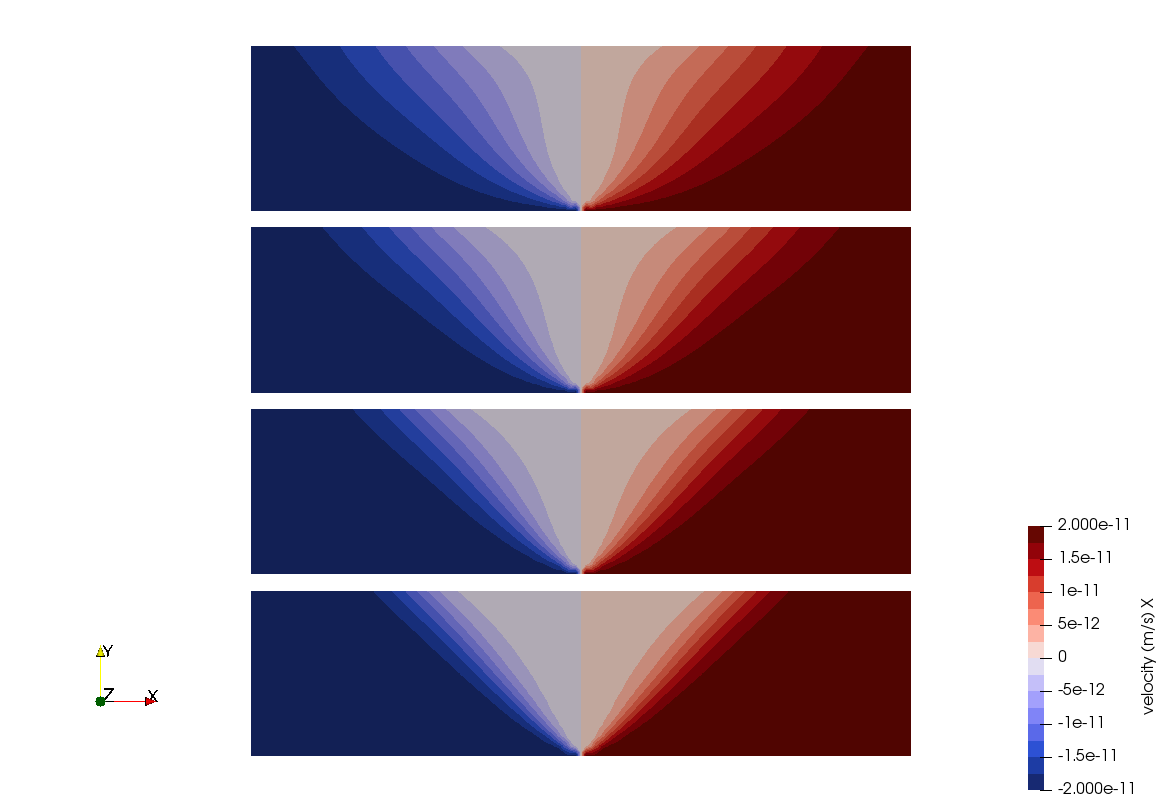
\includegraphics[width=5.7cm]{python_codes/fieldstone_87/results/experiment_02/u}
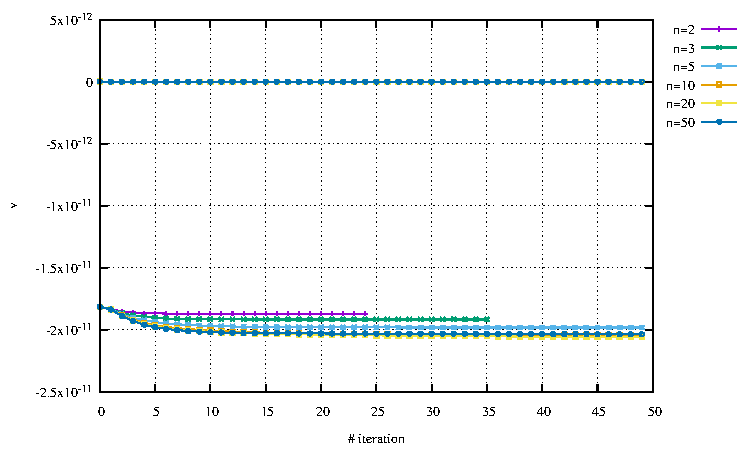
\includegraphics[width=5.7cm]{python_codes/fieldstone_87/results/experiment_02/v}
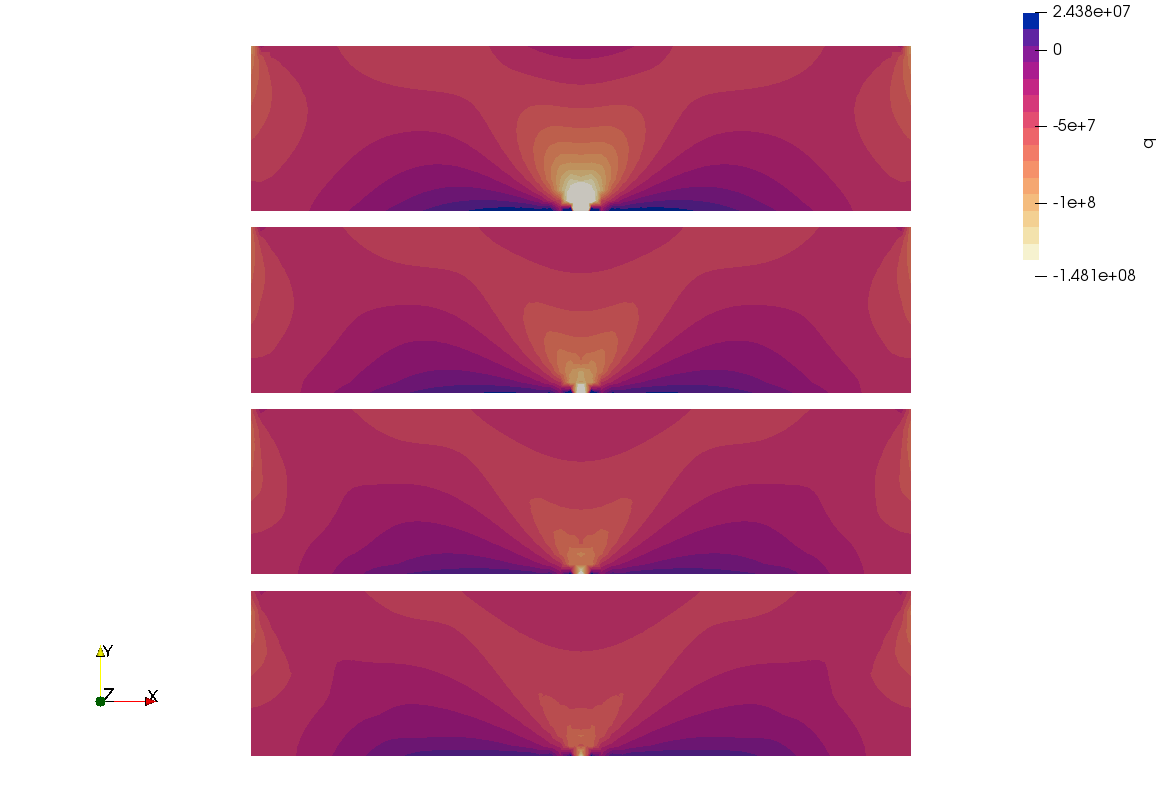
\includegraphics[width=5.7cm]{python_codes/fieldstone_87/results/experiment_02/p}\\
\end{center}

\begin{center}
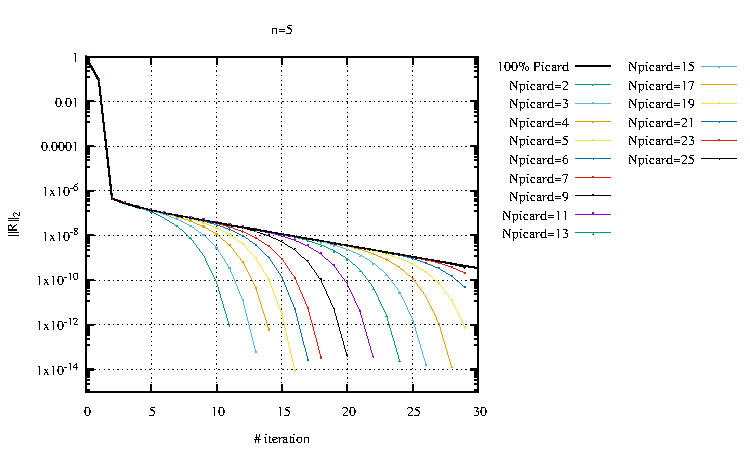
\includegraphics[width=7cm]{python_codes/fieldstone_87/results/experiment_02/conv_n5}
\includegraphics[width=7cm]{python_codes/fieldstone_87/results/experiment_02/conv_n10}\\
\includegraphics[width=7cm]{python_codes/fieldstone_87/results/experiment_02/theta_n5}
\includegraphics[width=7cm]{python_codes/fieldstone_87/results/experiment_02/theta_n10}\\
{\captionfont Influence of the number of Picard iterations before wtiching to Newton ones
for $n=5$ (left) and $n=10$ (right).}
\end{center}





\newpage
%--------------------------------------------------------------------------
\subsubsection*{Experiments 3 \& 4 - Slab detachment benchmark}

Two materials are present in the domain: the lithosphere (mat.1) and the mantle (mat.2):

\begin{center}
\includegraphics[width=7cm]{python_codes/fieldstone_87/images/drawing.png}\\
{\captionfont the top layer may or may not be there, depending on the chosen case, see below.}
\end{center}

The overriding plate is $80\si{\kilo\metre}$ thick and is placed at the top of the domain. 
An already subducted slab (also mat 1) of $250\si{\kilo\metre}$ length hangs vertically under this plate.
The mantle occupies the rest of the domain.
Several experiments with increasing levels of complexity have been designed 
and the first two ones are carried out for now.

\begin{itemize}
\item case 1a: 
The mantle has a constant viscosity $\eta_0=10^{21}\si{\pascal\second}$ and a density 
$\rho=3150\si{\kilogram\per\cubic\metre}$. 
The slab has a density $\rho=3300\si{\kilogram\per\cubic\metre}$ 
and is characterised by a power law rheology so that 
its effective viscosity depends on the effective strainrate $\dot\varepsilon_e$.
We set $n_s=4$ and $A=(2 \times 4.75\!\times\! 10^{11})^{-n_s}$ so that 
\begin{equation}
\eta_{eff}
=\frac{1}{2} A^{-1/n_s} \dot\varepsilon_e^{1/n_s-1} 
=\frac{1}{2} [(2 \times 4.75\!\times\! 10^{11})^{-n_s}]^{-1/n_s} \dot\varepsilon_e^{1/n_s-1} 
=4.75\!\times\! 10^{11} \dot\varepsilon_e^{1/n_s-1} 
= B \dot\varepsilon_e^\alpha
\end{equation}

\item case 1b: 
Both mantle and slab are have a power law rheology. 
The slab is the same as in case 1a, but the mantle rheology is now 
characterised by $A=(2 \times 4.54 \!\times\! 10^{10})^{-n_m}$ or $B=4.54 \times 10^{10}$ 
and $n_m=3$.

\item case 2a: same as case 1a, but the system now has a free surface. Depending on the code 
you are using, a conforming mesh or a sticky air approach can be used. If the sticky air option is chosen,
$40km$ of air are added at the top of the system and no boundary conditions are prescribed on 
the top of the domain. The choice of air viscosity is yours and you may wish to read \cite{crsg12}.
Ideally it should be low enough so that decreasing it even more does not alter the results. 

\item case 2b: same as case 2a, but with nonlinear mantle of case 1b. 

\end{itemize}

Boundary conditions are no-slip on the sides and free-slip on the top and bottom. 
Note that calculations are actually carried out with a density field to which the value 3150 has 
been subtracted, i.e. the lithosphere has a density of 150 while the mantle has zero density.
The regularisation parameter is set to $\dot{\gamma}=10^{-20}\si{\per\second}$.
Gravity is vertical and set to $-10\si{\metre\per\square\second}$.

\newpage
\underline{Case 1a (Experiment \#3)}

\begin{center}
\includegraphics[width=5.7cm]{python_codes/fieldstone_87/results/experiment_03/100x66_N/vel.png}
\includegraphics[width=5.7cm]{python_codes/fieldstone_87/results/experiment_03/100x66_N/p.png}
\includegraphics[width=5.7cm]{python_codes/fieldstone_87/results/experiment_03/100x66_N/sr.png}\\
\includegraphics[width=5.7cm]{python_codes/fieldstone_87/results/experiment_03/100x66_N/eta.png}
\includegraphics[width=5.7cm]{python_codes/fieldstone_87/results/experiment_03/100x66_N/etan.png}
\includegraphics[width=5.7cm]{python_codes/fieldstone_87/results/experiment_03/theta}\\
\includegraphics[width=5.7cm]{python_codes/fieldstone_87/results/experiment_03/conv}
\includegraphics[width=5.7cm]{python_codes/fieldstone_87/results/experiment_03/du}
\includegraphics[width=5.7cm]{python_codes/fieldstone_87/results/experiment_03/dp}\\
\includegraphics[width=5.7cm]{python_codes/fieldstone_87/results/experiment_03/u}
\includegraphics[width=5.7cm]{python_codes/fieldstone_87/results/experiment_03/v}
\includegraphics[width=5.7cm]{python_codes/fieldstone_87/results/experiment_03/p}\\
\includegraphics[width=5.7cm]{python_codes/fieldstone_87/results/experiment_03/horizontal_profile_eta.pdf}
\includegraphics[width=5.7cm]{python_codes/fieldstone_87/results/experiment_03/vertical_profile_eta.pdf}
\includegraphics[width=5.7cm]{python_codes/fieldstone_87/results/experiment_03/horizontal_profile_srn.pdf}\\
\includegraphics[width=5.7cm]{python_codes/fieldstone_87/results/experiment_03/vertical_profile_srn.pdf}
\includegraphics[width=5.7cm]{python_codes/fieldstone_87/results/experiment_03/horizontal_profile_p.pdf}
\includegraphics[width=5.7cm]{python_codes/fieldstone_87/results/experiment_03/vertical_profile_p.pdf}\\
\end{center}


\newpage
\underline{Case 1b (Experiment \#4)}

\begin{center}
\includegraphics[width=5.7cm]{python_codes/fieldstone_87/results/experiment_04/100x66_N/vel.png}
\includegraphics[width=5.7cm]{python_codes/fieldstone_87/results/experiment_04/100x66_N/p.png}
\includegraphics[width=5.7cm]{python_codes/fieldstone_87/results/experiment_04/100x66_N/sr.png}\\
\includegraphics[width=5.7cm]{python_codes/fieldstone_87/results/experiment_04/100x66_N/eta.png}
\includegraphics[width=5.7cm]{python_codes/fieldstone_87/results/experiment_04/100x66_N/etan.png}
\includegraphics[width=5.7cm]{python_codes/fieldstone_87/results/experiment_04/theta}\\
\includegraphics[width=5.7cm]{python_codes/fieldstone_87/results/experiment_04/conv}
\includegraphics[width=5.7cm]{python_codes/fieldstone_87/results/experiment_04/du}
\includegraphics[width=5.7cm]{python_codes/fieldstone_87/results/experiment_04/dp}\\
\includegraphics[width=5.7cm]{python_codes/fieldstone_87/results/experiment_04/u}
\includegraphics[width=5.7cm]{python_codes/fieldstone_87/results/experiment_04/v}
\includegraphics[width=5.7cm]{python_codes/fieldstone_87/results/experiment_04/p}\\
\includegraphics[width=5.7cm]{python_codes/fieldstone_87/results/experiment_04/horizontal_profile_eta.pdf}
\includegraphics[width=5.7cm]{python_codes/fieldstone_87/results/experiment_04/vertical_profile_eta.pdf}
\includegraphics[width=5.7cm]{python_codes/fieldstone_87/results/experiment_04/horizontal_profile_srn.pdf}\\
\includegraphics[width=5.7cm]{python_codes/fieldstone_87/results/experiment_04/vertical_profile_srn.pdf}
\includegraphics[width=5.7cm]{python_codes/fieldstone_87/results/experiment_04/horizontal_profile_p.pdf}
\includegraphics[width=5.7cm]{python_codes/fieldstone_87/results/experiment_04/vertical_profile_p.pdf}
\end{center}


\newpage
%-----------------------------------------------------------------------------
\subsubsection*{Experiment 5 - inclusion in linear matrix under simple shear}

The setup originates in Tenczer et al (2001) \cite{tesb01}. 
The domain is a unit square. In its middle a circular inclusion of radius $R=0.1$
is present. While the matrix is a Newtonian fluid, the inclusion is characterised
by a power law rheology. 
Boundary conditions are $\vec\upnu=(0.5,0)$ at the top, $\vec\upnu=(-0.5,0)$
at the bottom, and $v=0$ on the sides.
The background strain rate $\dot\varepsilon_{xy}$ is then given by
\[
\dot\varepsilon_{xy} = \frac{1}{2}\left( \frac{\partial u}{\partial y}+ \frac{\partial v}{\partial x} \right)
\simeq \frac{1}{2} \frac{\Delta u}{\Delta y}
= \frac{1}{2} \frac{0.5-(-0.5)}{1} = 0.5
\]
The authors use the BASIL finite element code (see Section~\ref{app:codes})
with a mesh based on triangles. We here however 
keep relying on quadrilateral elements so that the edges of the elements cannot be 
aligned with the material discontinuity. 
The material model is called at every quadrature point.  

In what follows we use a $64\times 64$ element mesh. 
We set $B=1$ and $n=1$ (i.e. $\alpha=0$) for the matrix, 
so that its viscosity is simply 1. The inclusion is characterised by $B=5$ and $n=\{1,2,3,4,5,10\}$.
Pressure is volume-average normalised. The regularisation parameter is set to $\dot{e}=10^{-5}$. 

\begin{center}
\includegraphics[width=8cm]{python_codes/fieldstone_87/results/experiment_05/u.png}
\includegraphics[width=8cm]{python_codes/fieldstone_87/results/experiment_05/v.png}\\
\includegraphics[width=8cm]{python_codes/fieldstone_87/results/experiment_05/vel.png}
\includegraphics[width=8cm]{python_codes/fieldstone_87/results/experiment_05/sr.png}\\
\includegraphics[width=8cm]{python_codes/fieldstone_87/results/experiment_05/press.png}
\includegraphics[width=8cm]{python_codes/fieldstone_87/results/experiment_05/eta.png}\\
{\captionfont From left to right: $n=1,2,3,4,5,10$. resolution 64x64. Newton.}
\end{center}

We see that when $n$ increases so does the effective viscosity in the inclusion. When 
$n$ becomes very large this experiment becomes very similar to the SolVi (see 
Section~\ref{sec:geobench}) benchmark.

\begin{center}
\includegraphics[width=7.8cm]{python_codes/fieldstone_87/results/experiment_05/conv_picard.pdf}
\includegraphics[width=7.8cm]{python_codes/fieldstone_87/results/experiment_05/conv_meth1.pdf}\\
\includegraphics[width=7.8cm]{python_codes/fieldstone_87/results/experiment_05/conv_meth2.pdf}
\includegraphics[width=7.8cm]{python_codes/fieldstone_87/results/experiment_05/conv_meth3.pdf}\\
{\captionfont Npicard =4. $\dot{e}=10^{-16}$}
\end{center}


\begin{center}
\includegraphics[width=5.7cm]{python_codes/fieldstone_87/results/experiment_05/diag_eta}
\includegraphics[width=5.7cm]{python_codes/fieldstone_87/results/experiment_05/diag_sr}
\includegraphics[width=5.7cm]{python_codes/fieldstone_87/results/experiment_05/diag_p}\\
\includegraphics[width=5.7cm]{python_codes/fieldstone_87/results/experiment_05/diag_u}
\includegraphics[width=5.7cm]{python_codes/fieldstone_87/results/experiment_05/diag_v}\\
{\captionfont Effective viscosity, strain rate and pressure along the diagonal in the 
upper right quadrant (i.e. $x\ge 0.5$ and $y\ge 0.5$)}
\end{center}

\begin{center}
\includegraphics[width=5.7cm]{python_codes/fieldstone_87/results/experiment_05/theta_meth2}
\includegraphics[width=5.7cm]{python_codes/fieldstone_87/results/experiment_05/theta_meth3}
\end{center}



\newpage
%--------------------------------------------------------------------------
\subsubsection*{Experiment 6 - the Stokes sphere}

This is a simple two-dimensional experiment in which a Stokes sphere is placed at coordinates 
$(L_x/2,L_y/2)$ and has a radius of 100\si{\kilo\metre}. 
The domain is $600\times600$\si{\kilo\metre}, 
gravity is set to $g_z=-9.81\si{\metre\per\square\second}$.
The temperature is a linear gradient between  $T=550\si{\celsius}$ 
at the surface and $T=1330\si{\celsius}$ at the bottom,
except in the sphere where it is set to a constant $T=550\si{\celsius}$.
The density of the surrounding mantle is $\rho_0=3000\si{\kilogram\per\cubic\meter}$ 
and the sphere reference density is $\rho_0=3300\si{\kilogram\per\cubic\meter}$. The thermal expansion 
coefficient is set to $\alpha=3\cdot 10^{-5} \si{\per\kelvin}$ and the reference temperature to $T_0=0\si{\celsius}$.
The density is given by: 
\[
\rho(T)=\rho_0(1-\alpha(T-T_0))
\]
Boundary conditions are free slip at the bottom and the sides, open at the top (free surface).

The rheology is of the dislocation creep type and the effective viscosity is then computed as follows:
\[
\eta 
= \frac{1}{2} A^{-\frac1n} \dot\varepsilon_e^{\frac1n-1}  \exp \frac{Q}{nRT} 
= \underbrace{ \frac{1}{2} A^{-\frac1n} \exp \frac{Q}{nRT} }_{B} \dot\varepsilon_e^{\alpha}  
\]
Note that we still use a regularisation parameter set to $\dot{e}=10^{-18}\si{\per\second}$, 
and that no viscosity cutoff is needed here. 


\begin{center}
\includegraphics[width=5.5cm]{python_codes/fieldstone_87/results/experiment_06/vel.png}
\includegraphics[width=5.5cm]{python_codes/fieldstone_87/results/experiment_06/u.png}
\includegraphics[width=5.5cm]{python_codes/fieldstone_87/results/experiment_06/v.png}\\
\includegraphics[width=5.5cm]{python_codes/fieldstone_87/results/experiment_06/sr.png}
\includegraphics[width=5.5cm]{python_codes/fieldstone_87/results/experiment_06/eta.png}
\includegraphics[width=5.5cm]{python_codes/fieldstone_87/results/experiment_06/p.png}\\
{\captionfont Velocity, strain rate, viscosity and pressure fields. 128x128 mesh.}
\end{center}

\begin{center}
\includegraphics[width=5.7cm]{python_codes/fieldstone_87/results/experiment_06/conv_48x48.pdf}
\includegraphics[width=5.7cm]{python_codes/fieldstone_87/results/experiment_06/conv_64x64.pdf}\\
\includegraphics[width=5.7cm]{python_codes/fieldstone_87/results/experiment_06/conv_80x80.pdf}
\includegraphics[width=5.7cm]{python_codes/fieldstone_87/results/experiment_06/conv_meth3.pdf}
\end{center}

\begin{center}
\includegraphics[width=7.3cm]{python_codes/fieldstone_87/results/experiment_06/horizontal_profile_uv}
\includegraphics[width=7.3cm]{python_codes/fieldstone_87/results/experiment_06/horizontal_profile_eta}\\
\includegraphics[width=7.3cm]{python_codes/fieldstone_87/results/experiment_06/horizontal_profile_sr}
\includegraphics[width=7.3cm]{python_codes/fieldstone_87/results/experiment_06/horizontal_profile_p}\\
\includegraphics[width=7.3cm]{python_codes/fieldstone_87/results/experiment_06/vertical_profile_uv}
\includegraphics[width=7.3cm]{python_codes/fieldstone_87/results/experiment_06/vertical_profile_eta}\\
\includegraphics[width=7.3cm]{python_codes/fieldstone_87/results/experiment_06/vertical_profile_sr}
\includegraphics[width=7.3cm]{python_codes/fieldstone_87/results/experiment_06/vertical_profile_p}\\
\end{center}



\newpage
%--------------------------------------------------------------------------
\subsubsection*{Experiment 7 - Deformation around a Fault that cuts a Block of Viscous Material}

The idea for this experiment comes from Barr \& houseman \cite{baho92,baho96}.


\begin{center}
\includegraphics[width=10cm]{python_codes/fieldstone_87/images/baho}\\
{\captionfont Taken from 
\url{http://homepages.see.leeds.ac.uk/~eargah/basil/exa_fault.html}: 
Here we show the calculated deformation field around a fault that cuts the right 
hand boundary of the block as far as the centre of the block.  The deformation field 
includes a singularity in the stress components at the fault tip.  For that reason, 
we concentrate mesh points around the fault-tip as shown in the upper left diagram, 
but the accuracy with which the deformation field is computed can be checked against 
an analytic solution for the crack tip.  The fault permits a displacement discontinuity 
parallel to its direction, but requires continuity in the perpendicular directions, 
as for a buried geological fault which separates distinct sliding blocks of rock.  
If the rock is hot enough (deep in the crust) it creeps like a viscous fluid. 
The two diagrams in the middle row show the variation of the two components of displacement rate: 
Ux and Uy.  In Ux, we see the transition between a distributed shear flow on the left to the 
discontinuous displacement on the right.  To balance the horizontal flow, there is also a minor 
component of vertical flow as shown with Uy.  With elapsed time finite deformation of the block 
is shown on the lower right diagram.  The variation of displacement and deformation along the fault 
is diagnostic of the stress vs strain-rate exponent of the viscous material. 
}
\end{center}

We do not necessarily wish to reproduce the results in these papers, but since the authors use a 
power-law rheology their setup is interesting to us here. 
Their fault is defined by the following boundary conditions:
(1) the normal stress across the fault is continuous;
(2) the velocity normal to the fault is continuous but
otherwise unconstrained;
(3) the shear stress on the fault is equal to some constant,
which is set to be zero.
This would require a bespoke mesh where the points on the fault would need to be represented by 2 sets
of velocity dofs. 
In order not to implement such a feature, we resort to a very thin sliver of weak Newtonian material 
at the fault, with a thickness $\delta_F$.
Given the geometry, we also implement a form of mesh adaptivity which consists in 
stretching the elements in both $x$ and $y$ directions so as to yield smaller 
elements towards the tip of the fault:

\begin{center}
\includegraphics[width=10cm]{python_codes/fieldstone_87/images/mesh}\\
{\captionfont Stretched mesh of 120$\times$51 elements. 
This unstretched mesh would have square elements of size 196m. After stretching, 
elements in the middle of the domain have a dimension of about 127m, while near the boundaries the
elements have a dimension of about 610m.}
\end{center}


For $n=1$ the matrix around the fault is Newtonian and the authors specify its viscosity
to be $\eta_0=10^{20}\si{\pascal\second}$. For $n>1$ the authors do not specify the 
value of $B$ but rather resort to an indirect and unpractical way. We therefore postulate
\[
B =  \eta_0 \dot\varepsilon_0^{-\alpha}
\]
so that the viscosity is then 
\[
\eta =  \eta_0 \left(\frac{\dot\varepsilon_e}{\dot\varepsilon_0}\right) ^\alpha
\]
where the reference strain rate $\dot\varepsilon_0$ is defined by the slip rate of the fault 
(i.e. $u_0=10\si{\milli\metre\per\year}$) divided by $L_y$.
Ideally the fault should have no viscosity but due to machine precision considerations 
we set it to $\eta_F=10^{16}\si{\pascal\second}$.

The fault has a length $R_0=10\si{\kilo\metre}$ and the domain is then $2R_0 \times R_0$. 
Boundary conditions are as follows:

\begin{center}
\includegraphics[width=4cm]{python_codes/fieldstone_87/images/baho92}\\
{\captionfont Boundary conditions. Taken from \cite{baho92}, in which the domain is square.
$+u_0/2$ is prescribed at the top, and $-u_0/2$ is prescribed at the bottom.
}
\end{center}

\begin{center}
\includegraphics[width=7.8cm]{python_codes/fieldstone_87/results/experiment_07/conv_picard.pdf}
\includegraphics[width=7.8cm]{python_codes/fieldstone_87/results/experiment_07/conv_meth1.pdf}\\
\includegraphics[width=7.8cm]{python_codes/fieldstone_87/results/experiment_07/conv_meth2.pdf}
\includegraphics[width=7.8cm]{python_codes/fieldstone_87/results/experiment_07/conv_meth3.pdf}\\
{\captionfont Npicard =4. $\dot{e}=10^{-16}$}
\end{center}

\begin{center}
\includegraphics[width=7.8cm]{python_codes/fieldstone_87/results/experiment_07/stats_etaq_meth3.pdf}
\includegraphics[width=7.8cm]{python_codes/fieldstone_87/results/experiment_07/vrms_meth3.pdf}
\end{center}


\begin{center}
\includegraphics[width=5.52cm]{python_codes/fieldstone_87/results/experiment_07/u}
\includegraphics[width=5.52cm]{python_codes/fieldstone_87/results/experiment_07/v}
\includegraphics[width=5.52cm]{python_codes/fieldstone_87/results/experiment_07/vel}\\
\includegraphics[width=5.52cm]{python_codes/fieldstone_87/results/experiment_07/eta}
\includegraphics[width=5.52cm]{python_codes/fieldstone_87/results/experiment_07/sr}
\includegraphics[width=5.52cm]{python_codes/fieldstone_87/results/experiment_07/press}\\
{\captionfont From top to bottom: n=1,2,3,5,10. Mesh 102x51}
\end{center}





\newpage
%--------------------------------------------------------------------------
\subsubsection*{Experiment 8 - Poiseuille flow}

Boundary conditions are no slip at the top and bottom, and no vertical 
velocity on the sides.
Neumann (pressure) boundary conditions are applied on the 
left and right boundaries: $p_L=1$, $p_R=-1$ respectively.
We set $B=1$, $L_x=2$, $L_y=1$. 
Resolution is 80x40. The regularisation parameter is set to $\dot{e}=10^{-8}$.

There is an analytical solution to this problem. 
In Gerya \cite{gery19}, the viscosity of the non-Newtonian flow is defined by the following rheological
equation formulated in term of second stress and strain rate invariants
\[
2 \dot\varepsilon_e = C_1 \sigma_e^n
\]
where $C_1$ is a constant. The effective viscosity is formulated 
as a function of second strain rate invariant
\[
\eta_{eff} = \frac{\sigma_e}{2\dot\varepsilon_e} 
= C_1^{-\frac1n} (2 \dot\varepsilon_e)^{\frac1n-1}
= \underbrace{C_1^{-\frac1n} 2^\alpha}_{B}  \dot\varepsilon_e^{\alpha}
\]
In this example we will set $C_1=2^{n-1}$. This has the advantage of setting $\eta=1$ at 
the top and bottom walls. The vertical component 
of the velocity is zero, while the horizontal component is 
given by 
\[
u(x,n)=\frac{C_1}{n+1} \left(\frac{p_R-p_L}{L_x}\right)^n  
\left(  \left(\frac{L_y}{2}\right)^{n+1} - \left| y -\frac{L_y}{2}\right|^{n+1} \right)
\]
the viscosity by
\[
\eta(y,n)=\frac{1}{C_1} \left( \frac{p_R-p_L}{L_x} y \right)^{1-n}
\]
and the pressure by 
\[
p(x)=\frac{p_R-p_L}{L_x}x+p_L
\]
In the Newtonian case of constant viscosity, then 
\[
u(y) = \frac{1}{2} \frac{p_R-p_L}{L_x } \frac{1}{\eta_0} (y^2-yH)
\]

When the viscosity is equal to 1 ($\alpha=0$) we recover the standard parabolic 
velocity profile and a linear pressure field.
When $n>1$ we see that the low strain rate in the middle of the flow
yields high viscosities and these quickly grow to untractable values. 
We therefore limit ourselves to $n=2,3,4,5$:

\begin{center}
\includegraphics[width=8cm]{python_codes/fieldstone_87/results/experiment_08/meth3/vel_profile}
\includegraphics[width=8cm]{python_codes/fieldstone_87/results/experiment_08/meth3/eta_profile}\\
\includegraphics[width=8cm]{python_codes/fieldstone_87/results/experiment_08/meth3/sr_profile}
\includegraphics[width=8cm]{python_codes/fieldstone_87/results/experiment_08/meth3/vrms}
\end{center}

\begin{center}
\includegraphics[width=7cm]{python_codes/fieldstone_87/results/experiment_08/conv_picard.pdf}
\includegraphics[width=7cm]{python_codes/fieldstone_87/results/experiment_08/conv_meth1.pdf}\\
\includegraphics[width=7cm]{python_codes/fieldstone_87/results/experiment_08/conv_meth2.pdf}
\includegraphics[width=7cm]{python_codes/fieldstone_87/results/experiment_08/conv_meth3.pdf}\\
{\captionfont Npicard =4}
\end{center}

\begin{center}
\includegraphics[width=5cm]{python_codes/fieldstone_87/results/experiment_08/vel}
\includegraphics[width=5cm]{python_codes/fieldstone_87/results/experiment_08/eta}
\includegraphics[width=5cm]{python_codes/fieldstone_87/results/experiment_08/sr}\\
{\captionfont From top to bottom: $n=1,2,3,4,5$.}
\end{center}

\newpage
%--------------------------------------------------------------------------
\subsubsection*{Experiment 9 - the punch problem}

The domain is $1\times0.5$. No-slip boundary conditions are prescribed on the left, right, and bottom 
boundaries. On the top boundary $\upnu=(0,-1)$ is prescribed for $|x-L_x/2|<0.123456$.
We set $\dot{e}=10^{-6}$ and $B=1$.
When $n >> 1$ then $\alpha \rightarrow -1$ and then the effective viscosity tends to 
\[
\eta_{eff} \rightarrow 
\frac{B}{\dot\varepsilon_e}
=
\frac{Y}{2\dot\varepsilon_e}
\] 
with $Y=2B$. This is the standard form for the viscosity rescaling method in (simple) plasticity.
If the regularisation parameter is present, then 
\[
\eta_{eff} \rightarrow 
\frac{Y}{2(\dot\varepsilon_e + \dot{e})}
\] 
with $Y=2B$. This is the standard form for the viscosity rescaling method in (simple) plasticity.
Interestingly, when $\dot{e} \sim \dot\varepsilon_e$ then the 
viscosity tends to $\sim B/\dot{e}$ which acts as a maximum viscosity (soft) limiter.
In this case, $B/\dot{e}=10^6$ and we see that the viscosity in the rigid regions tends towards this value.

\begin{center}
\includegraphics[width=7.8cm]{python_codes/fieldstone_87/results/experiment_09/conv_picard.pdf}
\includegraphics[width=7.8cm]{python_codes/fieldstone_87/results/experiment_09/conv_meth1.pdf}\\
\includegraphics[width=7.8cm]{python_codes/fieldstone_87/results/experiment_09/conv_meth2.pdf}
\includegraphics[width=7.8cm]{python_codes/fieldstone_87/results/experiment_09/conv_meth3.pdf}\\
{\captionfont Npicard =4}
\end{center}


\begin{center}
\includegraphics[width=5.8cm]{python_codes/fieldstone_87/results/experiment_09/meth3/u}
\includegraphics[width=5.8cm]{python_codes/fieldstone_87/results/experiment_09/meth3/v}
\includegraphics[width=5.8cm]{python_codes/fieldstone_87/results/experiment_09/meth3/vel}\\
\includegraphics[width=5.8cm]{python_codes/fieldstone_87/results/experiment_09/meth3/press}
\includegraphics[width=5.8cm]{python_codes/fieldstone_87/results/experiment_09/meth3/sr}
\includegraphics[width=5.8cm]{python_codes/fieldstone_87/results/experiment_09/meth3/eta}\\
{\captionfont Resolution 80x40. $n=2,5,10,20,50,100$. Npicard=4. 
$\theta$ method 3. When $n>>1$ we indeed recover the 
classical solution of the rigid-plastic punch, see Section~\ref{sec:punch}}
\end{center}


\begin{center}
a)\includegraphics[width=7.38cm]{python_codes/fieldstone_87/results/experiment_09/surface_profile_u_meth3.pdf}
b)\includegraphics[width=7.38cm]{python_codes/fieldstone_87/results/experiment_09/surface_profile_v_meth3.pdf}\\
c)\includegraphics[width=7.38cm]{python_codes/fieldstone_87/results/experiment_09/surface_profile_sr_meth3.pdf}
d)\includegraphics[width=7.38cm]{python_codes/fieldstone_87/results/experiment_09/surface_profile_eta_meth3.pdf}\\
e)\includegraphics[width=7.38cm]{python_codes/fieldstone_87/results/experiment_09/surface_profile_p_meth3.pdf}\\
{\captionfont a,b,c,d,e) Velocity, strain rate, viscosity and pressure measured at the top of the domain, 
Npicard=4, 80x40.}
\end{center}

\begin{center}
\includegraphics[width=7cm]{python_codes/fieldstone_87/results/experiment_09/vrms_meth3.pdf}
\includegraphics[width=7cm]{python_codes/fieldstone_87/results/experiment_09/stats_etaq_meth3.pdf}\\
\includegraphics[width=7cm]{python_codes/fieldstone_87/results/experiment_09/theta_meth2.pdf}
\includegraphics[width=7cm]{python_codes/fieldstone_87/results/experiment_09/theta_meth3.pdf}\\
{\captionfont Npicard =4, $\theta$-method}
\end{center}


\newpage
%--------------------------------------------------------------------------
\subsubsection*{Experiment 10 - Spiegelman et al (2016) brick}



This experiment is presented in Spiegelman (2016) \cite{spmw16} and is also carried out 
in Fraters et al (2019) \cite{frbt19}. 
The domain is $120\times30\si{\kilo\metre}$. Since the rheology does not 
depend on pressure we set $\vec{g}=\vec{0}$.
Boundary conditions and material parameters are shown hereunder:
\begin{center}
\includegraphics[width=8cm]{python_codes/fieldstone_87/images/spmw16a}
\includegraphics[width=8cm]{python_codes/fieldstone_87/images/spmw16b}\\
\end{center}
The background strain rate is then 
\[
e = \frac{2 U_0}{L_x} = \frac{0.005 \si{\metre\per\year}}{120 \si{\kilo\metre}} \simeq 1.32\cdot 10^{-15} \si{\per\second}
\]
Although the rounded edges of the weak seed are implemented they are not 'seen' because 
of the low resolution: $r=0.02H=600\si{\meter}$ while the resolution we use here is $\sim 1200\si{\meter}$

In the von Mises rheology case (no pressure dependence), the viscosity of the top layer is given by 
\[
\eta_p= \frac{C}{2 \dot{\epsilon}_{e}}
\]
which we can replace by the following power law formulation:
$\eta = B \dot{\varepsilon}_e^\alpha$
where $B = \frac{\eta_{lim}}{e^\alpha}$ and $e=10^{-15}s^{-1}$ and $\eta_{lim}=C/2e$. 

\begin{center}
\includegraphics[width=7cm]{python_codes/fieldstone_87/results/experiment_10/conv_picard.pdf}
\includegraphics[width=7cm]{python_codes/fieldstone_87/results/experiment_10/conv_meth1.pdf}\\
\includegraphics[width=7cm]{python_codes/fieldstone_87/results/experiment_10/conv_meth2.pdf}
\includegraphics[width=7cm]{python_codes/fieldstone_87/results/experiment_10/conv_meth3.pdf}\\
{\captionfont Npicard =4}
\end{center}

\begin{center}
\includegraphics[width=7cm]{python_codes/fieldstone_87/results/experiment_10/vrms_meth3.pdf}
\includegraphics[width=7cm]{python_codes/fieldstone_87/results/experiment_10/stats_etaq_meth3.pdf}\\
\includegraphics[width=7cm]{python_codes/fieldstone_87/results/experiment_10/theta_meth2.pdf}
\includegraphics[width=7cm]{python_codes/fieldstone_87/results/experiment_10/theta_meth3.pdf}\\
{\captionfont Npicard =4, $\theta$-method}
\end{center}


\begin{center}
\includegraphics[width=5.7cm]{python_codes/fieldstone_87/results/experiment_10/meth3/vel}
\includegraphics[width=5.7cm]{python_codes/fieldstone_87/results/experiment_10/meth3/u}
\includegraphics[width=5.7cm]{python_codes/fieldstone_87/results/experiment_10/meth3/v}\\
\includegraphics[width=5.7cm]{python_codes/fieldstone_87/results/experiment_10/meth3/press}
\includegraphics[width=5.7cm]{python_codes/fieldstone_87/results/experiment_10/meth3/sr}
\includegraphics[width=5.7cm]{python_codes/fieldstone_87/results/experiment_10/meth3/eta}\\
{\captionfont Npicard=4, $\theta$-method=3, resolution 100x25, $n=100$.}
\end{center}

\begin{center}
\includegraphics[width=16cm]{python_codes/fieldstone_87/images/fig1}\\
\includegraphics[width=14cm]{python_codes/fieldstone_87/images/fig2}\\
{\captionfont Taken from Spiegelman et al. Note that I am 99\% sure that the pressure range in the paper is wrong.}\\
\includegraphics[width=5.7cm]{python_codes/fieldstone_87/results/experiment_10/meth3/sr2}
\includegraphics[width=5.7cm]{python_codes/fieldstone_87/results/experiment_10/meth3/eta2}
\includegraphics[width=5.7cm]{python_codes/fieldstone_87/results/experiment_10/meth3/press2}\\
{\captionfont Same as above but with coloscales of Spiegelman et al} 
\end{center}





\newpage
%--------------------------------------------------------------------------
\subsubsection*{Flow around a cylinder}

Because of symmetries we model only one fourth of the system.
The domain is 4x8 and the cylinder is centered on the origin with a radius of 1/2.
Free slip boundary conditions are prescribed on the sides, and $\vec\upnu=(0,-1)$
is prescribed at the top. There is no gravity so density is irrelevant. 

We start with a power-law rheology, with $B=1$ and $n=5$ , $\dot{e}=10^{-4}$:
\begin{center}
\includegraphics[width=7.64cm]{python_codes/fieldstone_87/results/experiment_11/meth3/u}
\includegraphics[width=7.64cm]{python_codes/fieldstone_87/results/experiment_11/meth3/v}\\
\includegraphics[width=7.64cm]{python_codes/fieldstone_87/results/experiment_11/meth3/vel}
\includegraphics[width=7.64cm]{python_codes/fieldstone_87/results/experiment_11/meth3/press}\\
\includegraphics[width=7.64cm]{python_codes/fieldstone_87/results/experiment_11/meth3/sr}
\includegraphics[width=7.64cm]{python_codes/fieldstone_87/results/experiment_11/meth3/eta}\\
{\captionfont Resolution 40x80. Npicard=4. $\theta$ method 3. }
\end{center}

\begin{center}
\includegraphics[width=7.5cm]{python_codes/fieldstone_87/results/experiment_11/conv_picard.pdf}
\includegraphics[width=7.5cm]{python_codes/fieldstone_87/results/experiment_11/conv_meth1.pdf}\\
\includegraphics[width=7.5cm]{python_codes/fieldstone_87/results/experiment_11/conv_meth2.pdf}
\includegraphics[width=7.5cm]{python_codes/fieldstone_87/results/experiment_11/conv_meth3.pdf}
\end{center}

\begin{center}
\includegraphics[width=7.5cm]{python_codes/fieldstone_87/results/experiment_11/bottom_profile_eta.pdf}
\includegraphics[width=7.5cm]{python_codes/fieldstone_87/results/experiment_11/bottom_profile_sr.pdf}
\includegraphics[width=7.5cm]{python_codes/fieldstone_87/results/experiment_11/bottom_profile_v.pdf}
\includegraphics[width=7.5cm]{python_codes/fieldstone_87/results/experiment_11/bottom_profile_p.pdf}\\
{\captionfont Measurements at $y=0$. $\theta$-method=3.}
\end{center}

\begin{center}
\includegraphics[width=7.5cm]{python_codes/fieldstone_87/results/experiment_11/vrms_meth3.pdf}
\includegraphics[width=7.5cm]{python_codes/fieldstone_87/results/experiment_11/stats_etaq_meth3.pdf}
\end{center}

TODO: The Herschel-Bulkley viscosity is given by
\[
\eta 
= K \dot{\varepsilon}_e^{\tilde{n}-1} + \frac{\tau_0}{\dot\varepsilon_e}
\]
and it is often regularised for small strain rates as follows:
\[
\eta 
= K \dot{\varepsilon}_e^{\tilde{n}-1} + \frac{\tau_0}{\dot\varepsilon_e}
\left(
1 - \exp \frac{\dot\varepsilon_e}{\dot\varepsilon_0}
\right)
\]
The Oldroyd number (Od) is used to quantify
the relation between the plastic and viscous effects.
\cite{demj04}
\[
Od =  \frac{\tau_0}{K (U/2r)^n}
\]
By choosing $K=1$, $U=1$, $r=1/2$ then $Od=\tau_0$. 
There remains to choose $\dot\varepsilon_0$. When $\dot\varepsilon_e \rightarrow 0$,
then $\eta \rightarrow \rightarrow K \dot{\varepsilon}_e^{\tilde{n}-1} + \tau_0/\dot\varepsilon_0$.



Vary Od from 0.1 to 100 




\newpage

\Literature: \textcite{russ20} \textcite{spmw16}

Remaining questions

- how to choose reg parameter

- how to measure convergence ?

- line search - ask Menno

- todo : 
  - carreau example
  - harmonic avrg example
  - vrm example

- higher order newton

- regularisation parameter or max viscosity ?

- positive definite

